\documentclass[aspectratio=169]{beamer}
\usepackage[utf8]{inputenc}
\usepackage{hyperref}
\usepackage{amsmath,amsfonts,amsthm,bm}
\usepackage{color}
\usepackage{graphicx} % Allows including images
\usepackage{subcaption}
\usepackage{booktabs} % Allows the use of \toprule, \midrule and \bottomrule in tables
\usepackage{tikz}
\usetikzlibrary{automata,positioning,shapes.geometric,shapes.misc,arrows}
%\usepackage{pgfplots}
\usepackage{listings}
\usepackage{courier}
\usepackage[version=4]{mhchem}
\usepackage{array}

\lstset{ %
    basicstyle=\scriptsize\ttfamily, % fonts that are used for the code
    breakatwhitespace=false,         % sets if automatic breaks should only happen at whitespace
%breaklines=true,                 % sets automatic line breaking
%captionpos=b,                    % sets the caption-position to bottom
    commentstyle=\color{gray}\textit,    % comment style
    keepspaces=true,                 % keeps spaces in text, useful for keeping indentation of code (possibly needs columns=flexible)
    keywordstyle=\color{blue},       % keyword style
    language=Python,                 % the language of the code
%otherkeywords={*,...},          % if you want to add more keywords to the set
    rulecolor=\color{black},         % if not set, the frame-color may be changed on line-breaks within not-black text (e.g. comments (green here))
    showspaces=false,                % show spaces everywhere adding particular underscores; it overrides 'showstringspaces'
    showstringspaces=false,          % underline spaces within strings only
    showtabs=false,                  % show tabs within strings adding particular underscores
    stringstyle=\color{red}, % string literal style
    tabsize=4,                       % sets default tabsize to 2 spaces
    columns=fixed                    % Using fixed column width (for e.g. nice alignment)
}

\hypersetup{
    colorlinks=true,
    linkcolor=red,
    filecolor=magenta,
    urlcolor=red,
}

\DeclareMathOperator*{\argmax}{argmax}
\DeclareMathOperator*{\argmin}{argmin}
\let \vec \mathbf

\newcommand{\classname}{NANO266}
\newcommand{\classyear}{Fall 2024}
\mode<presentation> {
    \usetheme{CambridgeUS}
    \setbeamertemplate{footline}[text line]{%
        \parbox{\linewidth}{\vspace*{-8pt}\classname\hfill\classyear\hfill\insertpagenumber}}

    %\setbeamertemplate{footline}[page number]
    \setbeamertemplate{navigation symbols}{}
}


\title[\classname Surfaces and Interfaces]{\classname~- Quantum Mechanical Modeling of Materials and Nanostructures\\Surfaces and Interfaces}

\author{Shyue Ping Ong}
\institute[UCSD]{University of California, San Diego\\
\medskip
}
\date{\classyear} % Date, can be changed to a custom date

\begin{document}


    \begin{frame}
        \titlepage % Print the title page as the first slide
    \end{frame}


    \begin{frame}{Modelling surfaces with the Supercell method}

        \begin{figure}
            \centering
            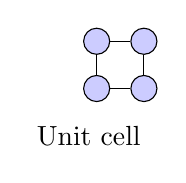
\begin{tikzpicture}[scale=0.5,
                atom/.style={circle,draw=black,fill=white!80!blue,minimum size=5},
                dopant/.style={circle,draw=black,fill=white!80!red,minimum size=5}
            ]
                \foreach \i in {1,...,2}
                    {
                    \foreach \j in {1,...,2}
                        {
                        \pgfmathtruncatemacro{\label}{\i\j};
                        \node[atom] (\label) at (1.2*\i,1.2*\j) { };

                    }
                }
% These draw commands are working as intended.
                \draw (11) -- (12);
                \draw (12) -- (22);
                \draw (21) -- (22);
                \draw (11) -- (21);
                \node at (1, 0) { Unit cell };

            \end{tikzpicture}
        \end{figure}

    \end{frame}


    \begin{frame}{Modelling surfaces with the Supercell method}

        \begin{figure}
            \centering
            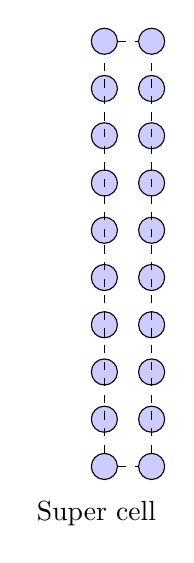
\begin{tikzpicture}[scale=0.5,
                atom/.style={circle,draw=black,fill=white!80!blue,minimum size=5},
                dopant/.style={circle,draw=black,fill=white!80!red,minimum size=5}
            ]
                \foreach \i in {1,...,2}
                    {
                    \foreach \j in {1,...,10}
                        {
                        \pgfmathtruncatemacro{\label}{\i\j};
                        \node[atom] (\label) at (1.2*\i,1.2*\j) { };
                    }
                }
                \draw[dashed] (11) -- (110);
                \draw[dashed] (11) -- (21);
                \draw[dashed] (21) -- (210);
                \draw[dashed] (110) -- (210);
                \node at (1, 0) { Super cell };

            \end{tikzpicture}
        \end{figure}

    \end{frame}


    \begin{frame}{Modelling surfaces with the Supercell method}

        \begin{figure}
            \centering
            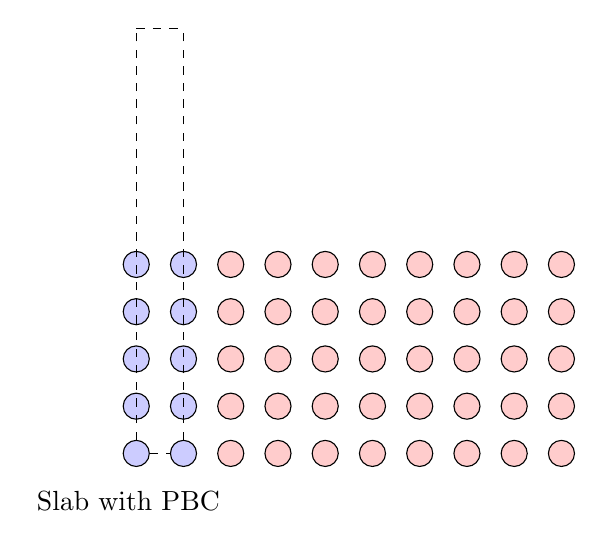
\begin{tikzpicture}[scale=0.5,
                atom/.style={circle,draw=black,fill=white!80!blue,minimum size=5},
                dopant/.style={circle,draw=black,fill=white!80!red,minimum size=5}
            ]
                \foreach \i in {1,...,2}
                    {
                    \foreach \j in {1,...,5}
                        {
                        \pgfmathtruncatemacro{\label}{\i\j};
                        \node[atom] (\label) at (1.2*\i,1.2*\j) { };
                    }
                }
                \foreach \i in {3,...,10}
                    {
                    \foreach \j in {1,...,5}
                        {
                        \pgfmathtruncatemacro{\label}{\i\j};
                        \node[dopant] (\label) at (1.2*\i,1.2*\j) { };
                    }
                }
                \draw[dashed] (11) -- (1.2,12);
                \draw[dashed] (11) -- (21);
                \draw[dashed] (21) -- (2.4,12);
                \draw[dashed] (1.2,12) -- (2.4,12);
                \node at (1, 0) { Slab with PBC };

            \end{tikzpicture}
        \end{figure}

    \end{frame}


    \begin{frame}{Lattice Planes}
        A lattice plane of a given Bravais lattice is a plane (or family of parallel planes) whose intersections with the lattice are periodic (i.e., are described by 2D Bravais nets) and intersect the Bravais lattice; equivalently, a lattice plane is any plane containing at least three noncollinear Bravais lattice points.
        \begin{figure}
            \centering
            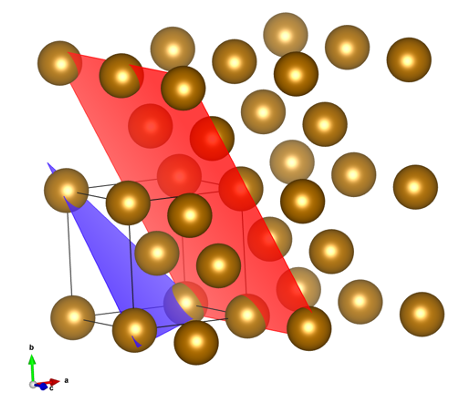
\includegraphics[width=0.3\linewidth]{lectures/figures/11_lattice_planes.png}
        \end{figure}
    \end{frame}

    \begin{frame}{Miller Indices}
        Lattice planes are represented by Miller indices, denoted as $(hkl)$, where $h$, $k$ and $l$ are integers.
        \begin{figure}
            \centering
            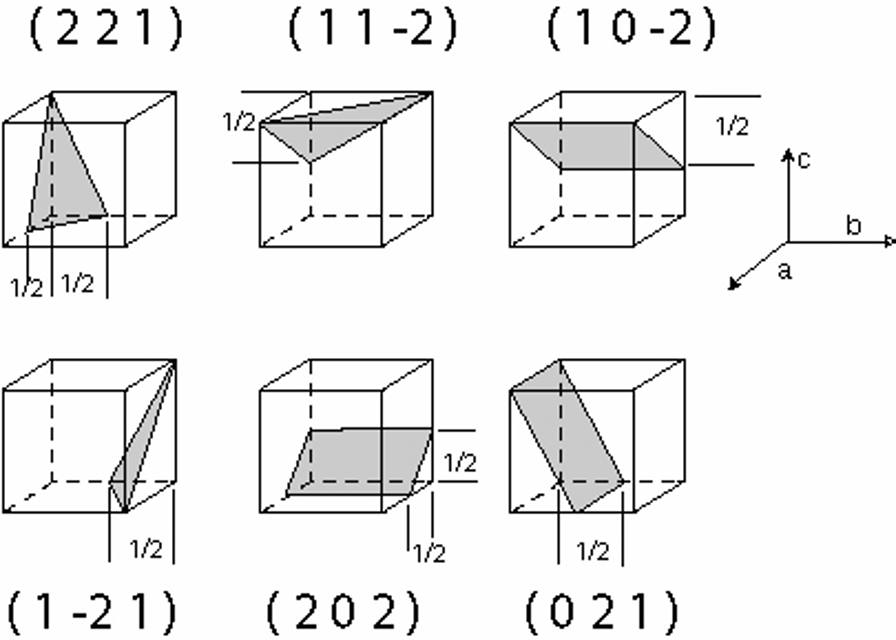
\includegraphics[width=0.5\linewidth]{lectures/figures/11_miller_indices.png}
        \end{figure}
    \end{frame}

    \begin{frame}{Surface Construction}
        \begin{columns}
            \column{0.5\textwidth}
            \begin{figure}
                \centering
                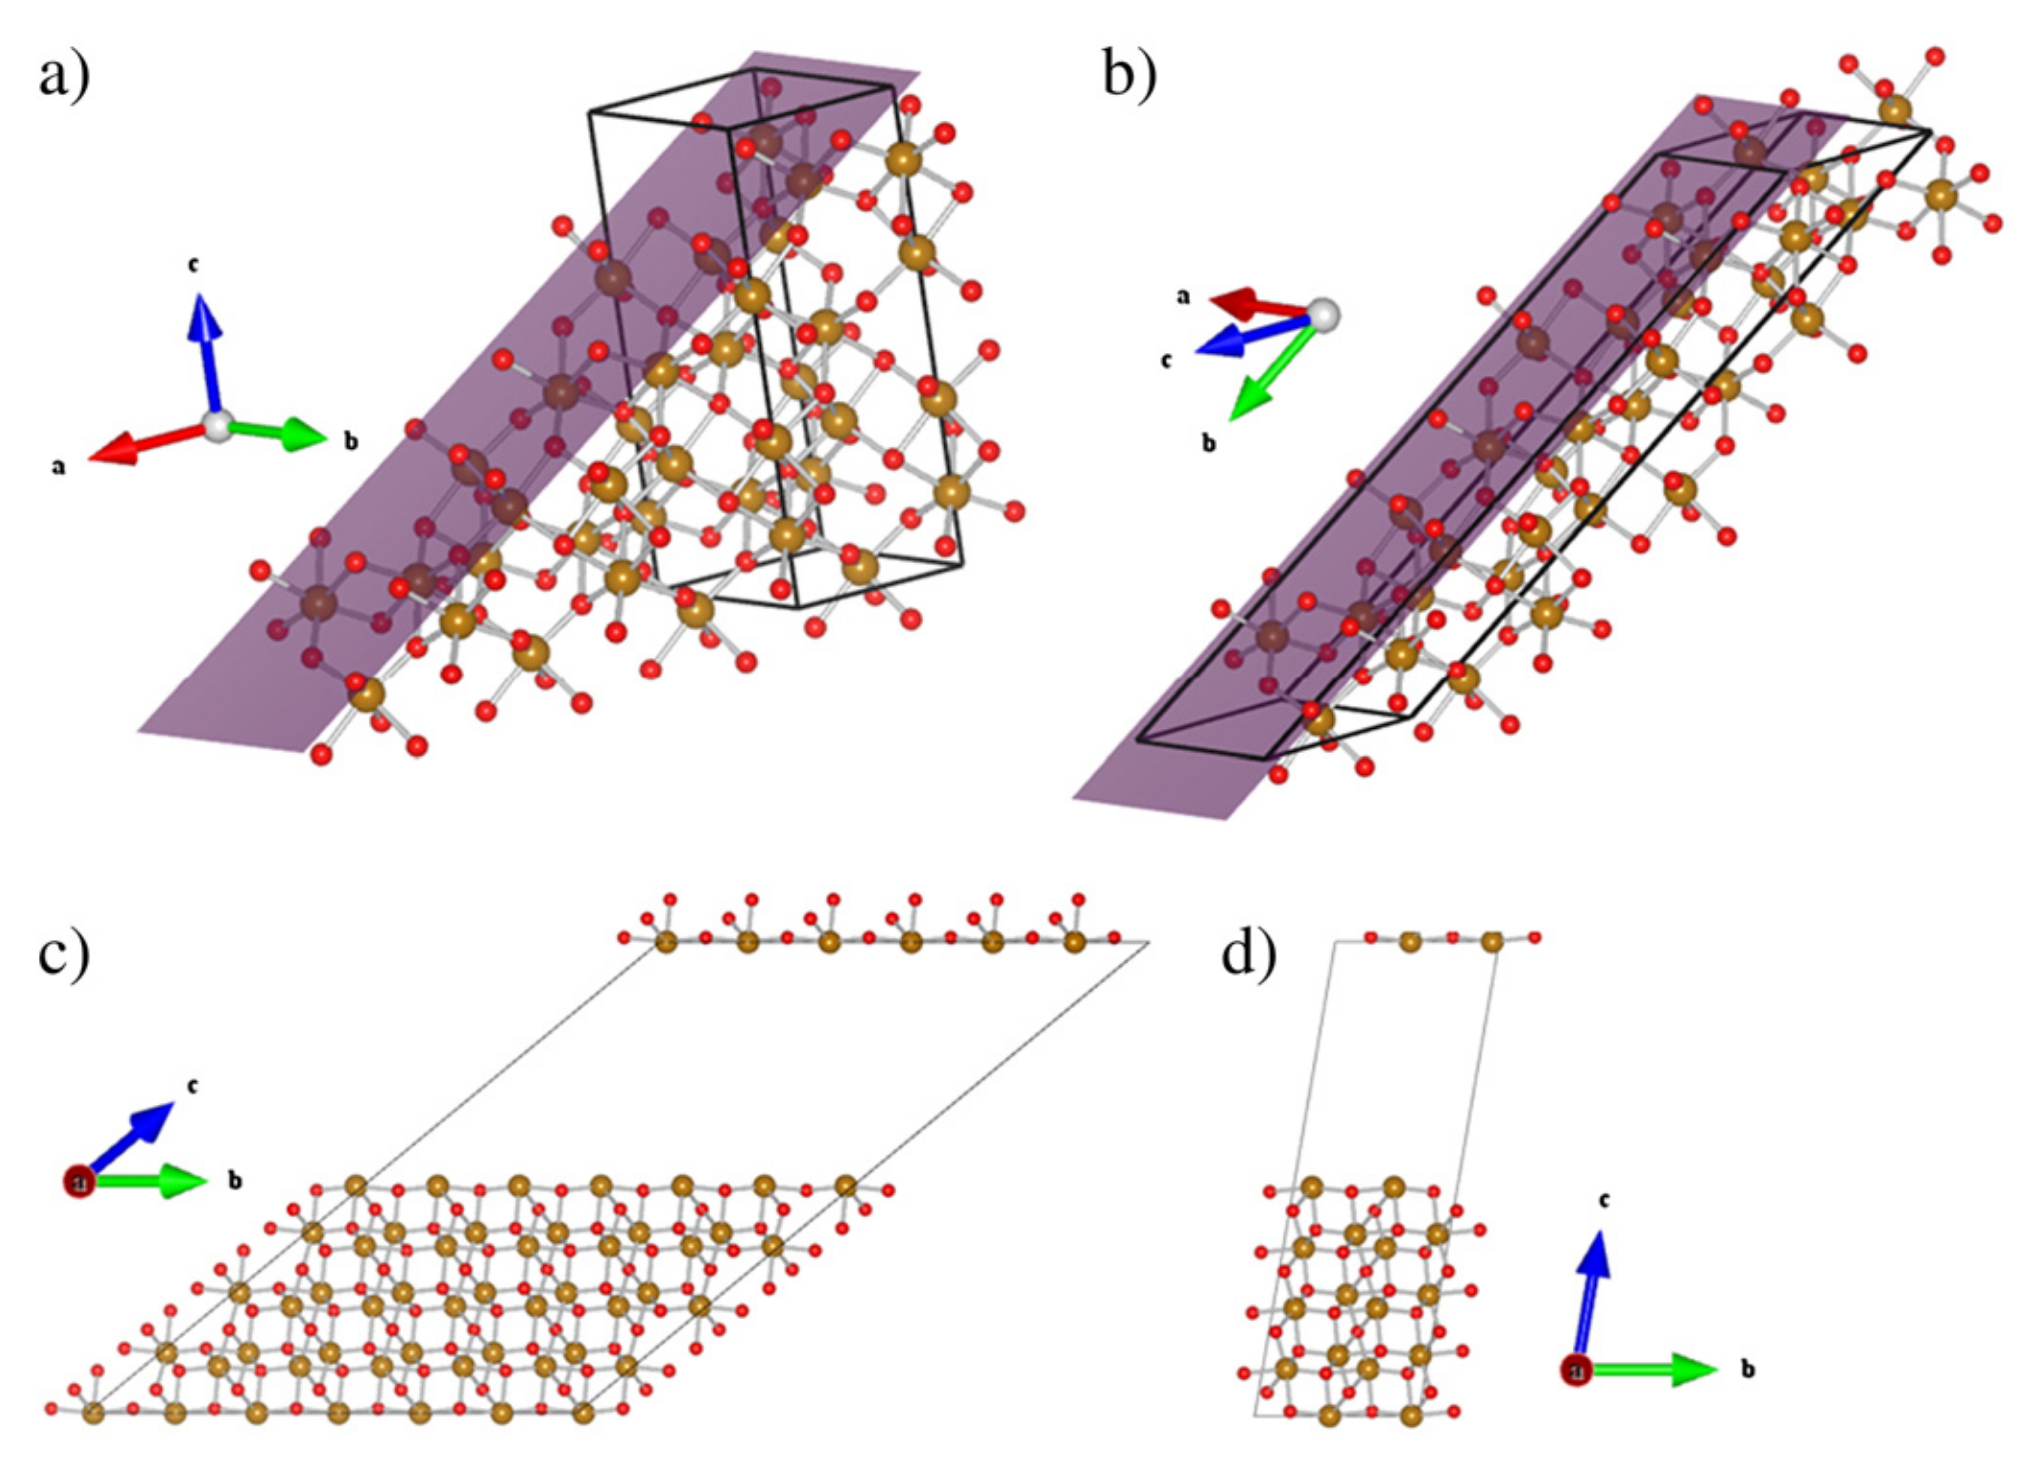
\includegraphics[width=\linewidth]{lectures/figures/11_surface_construction.png}
                \caption{Constructing the non-polar termination of the $(10\bar{1}4)$ surface of \ce{$\alpha$-Fe2O3}.\cite{sunEfficientCreationConvergence2013}}
            \end{figure}
            \column{0.5\textwidth}
            Steps
            \begin{enumerate}
                \item The bulk unit cell is basis-transformed such that the $(001)$ plane of the new basis is coplanar with the desired surface.
                \item The transformed surface-oriented basis is extended using the supercell slab construction to create a surface slab with vacuum.
                \item The slab is reduced by symmetry to a primitive surface unit cell.
            \end{enumerate}
        \end{columns}

    \end{frame}

    \begin{frame}{Key considerations of surface structures}
        \begin{enumerate}
            \item Which termination?
            \item Is the termination polar?
            \item Does surface reconstruction occur?
        \end{enumerate}

    \end{frame}

    \begin{frame}{Surface terminations}
        \begin{itemize}
            \item Symmetrically unique
            \item Most terminations break bonds – how many and which ones?
        \end{itemize}

        \begin{figure}
            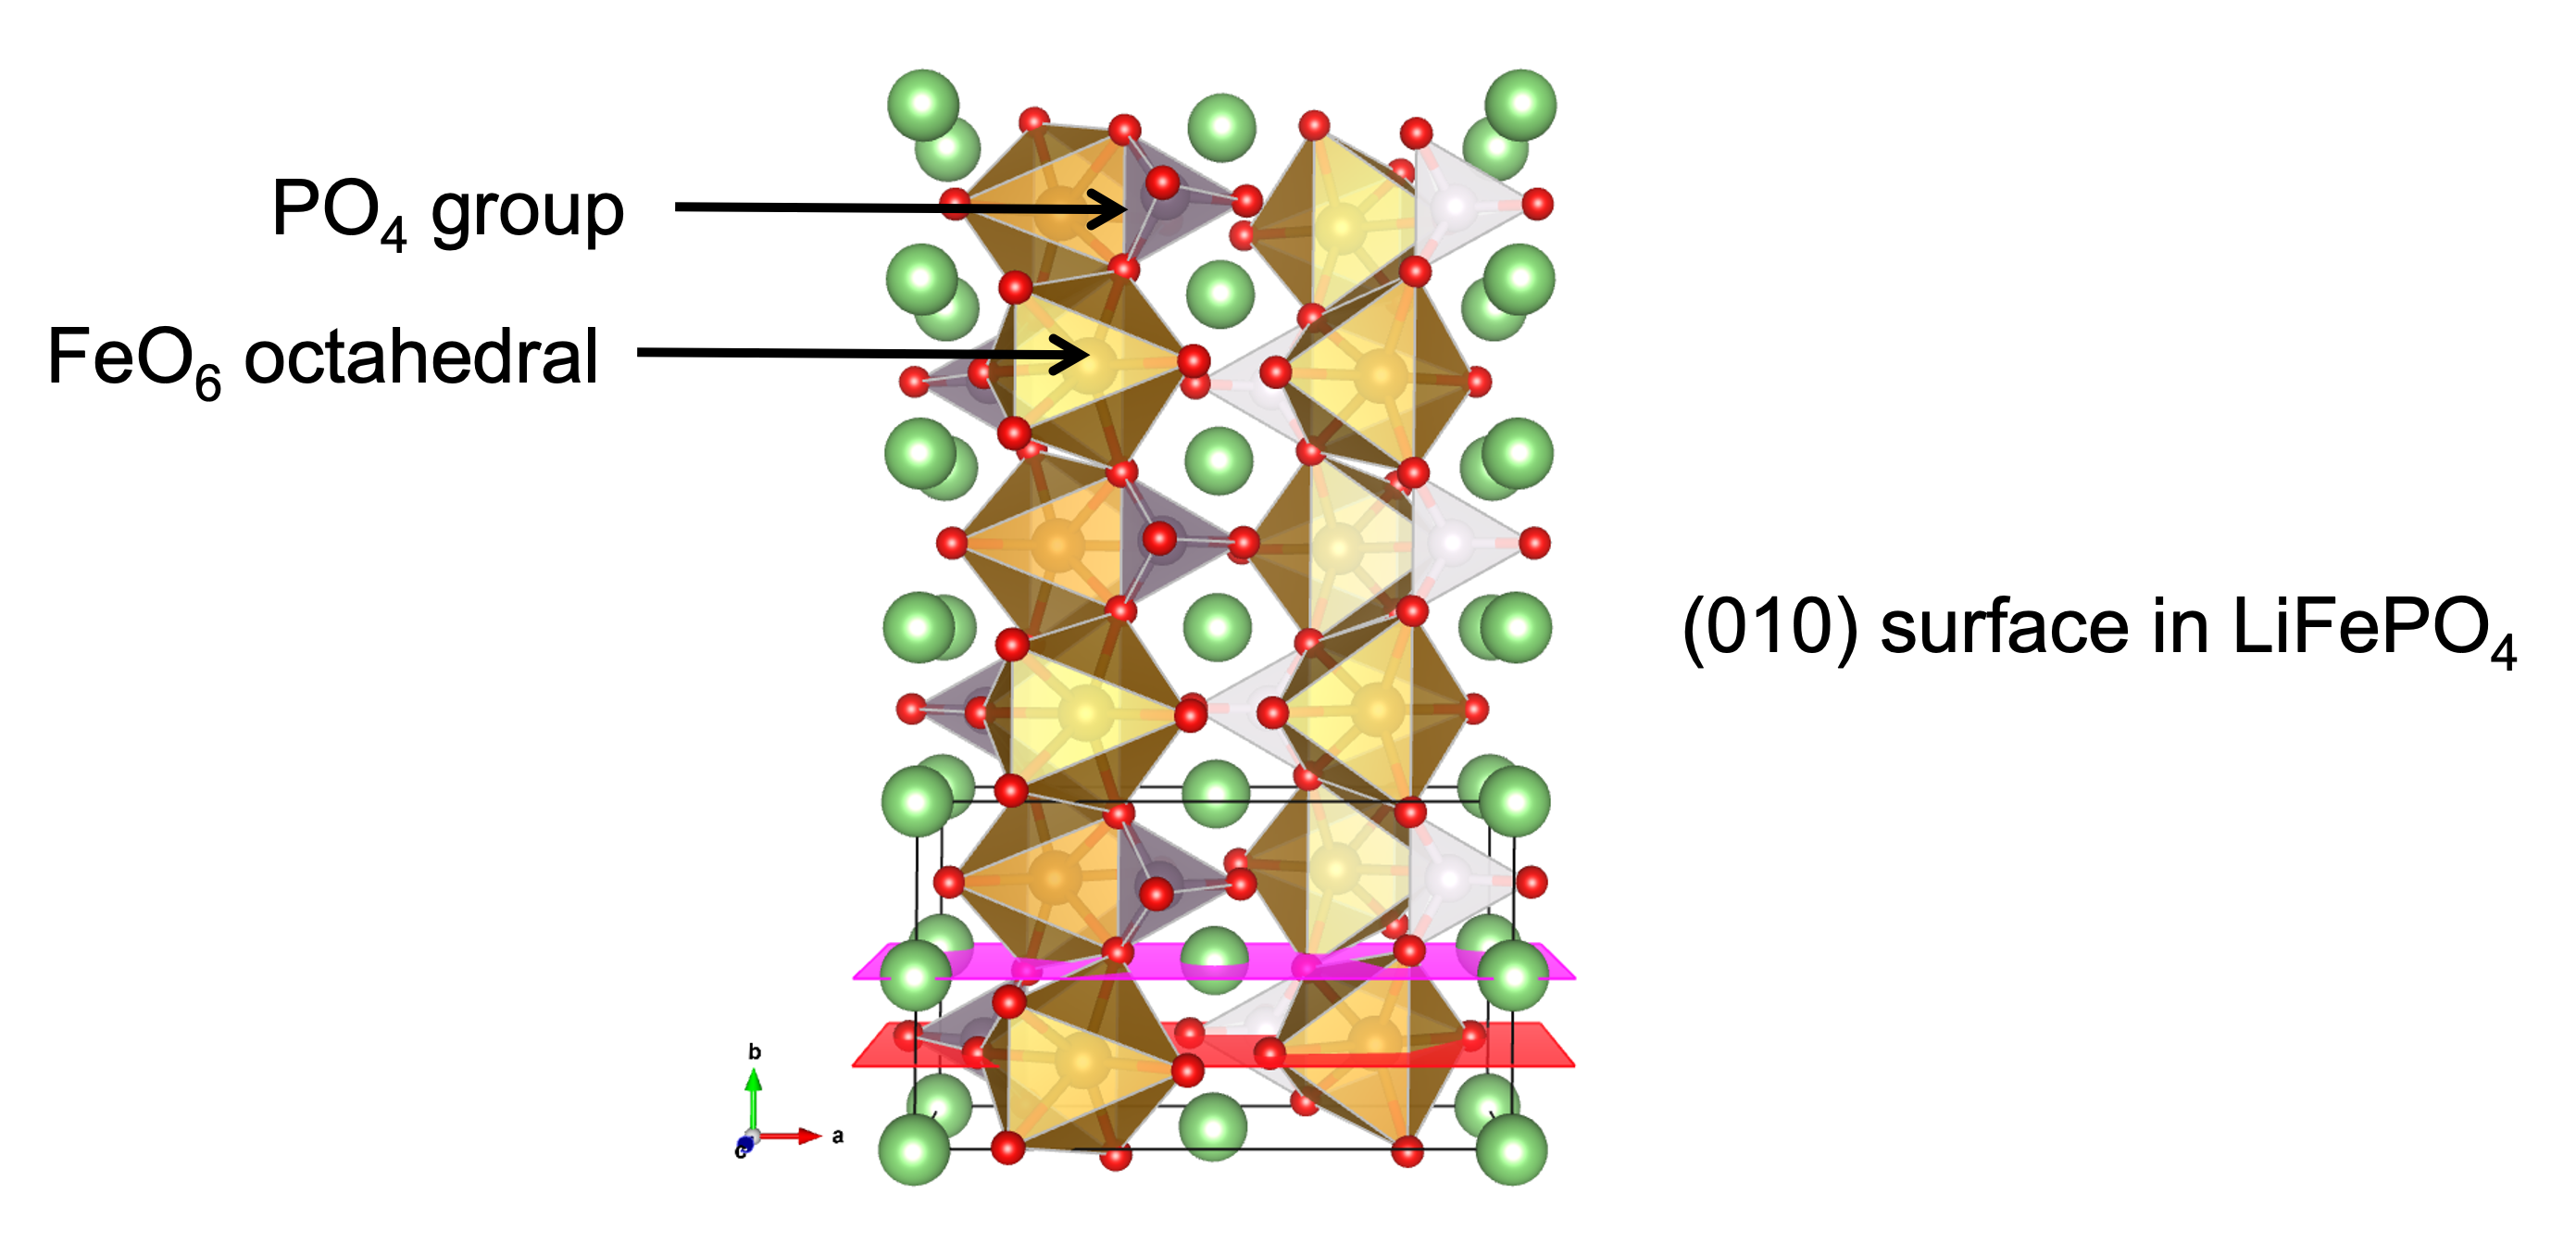
\includegraphics[width=0.7\linewidth]{lectures/figures/11_LFP_terminations.png}
        \end{figure}

    \end{frame}


    \begin{frame}{Tasker Classification}
        \begin{figure}
            \centering
            \begin{subfigure}{0.3\textwidth}
                \centering
                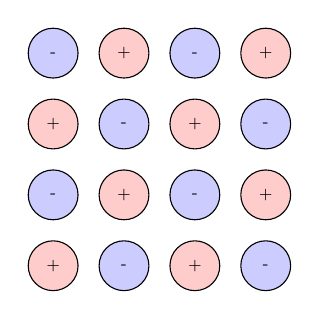
\begin{tikzpicture}[scale=0.9,
                    cation/.style={circle,draw=black,fill=white!80!red,minimum size=18},
                    anion/.style={circle,draw=black,fill=white!80!blue,minimum size=18}
                ]
                    \foreach \i in {1,...,2}
                        {
                        \foreach \j in {1,...,2}
                            {
                            \node[cation] (\i\j+) at (2*\i,2*\j) {\tiny{+}};
                            \node[anion] (\i\j+) at (2*\i,2*\j+1) {\tiny{-}};
                            \node[anion] (\i\j-) at (2*\i+1,2*\j) {\tiny{-}};
                            \node[cation] (\i\j-) at (2*\i+1,2*\j+1) {\tiny{+}};
                        }
                    }
                \end{tikzpicture}
                \caption{Type I (e.g., NaCl (100))}
            \end{subfigure}
            \begin{subfigure}{0.3\textwidth}
                \centering
                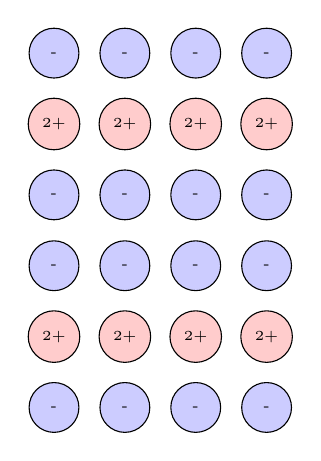
\begin{tikzpicture}[scale=0.9,
                    cation/.style={circle,draw=black,fill=white!80!red,minimum size=18},
                    anion/.style={circle,draw=black,fill=white!80!blue,minimum size=18}
                ]
                    \foreach \i in {1,...,4}
                        {
                        \node[anion] (II-) at (\i,0) {\tiny{-}};
                        \node[cation] (II+) at (\i,1) {\tiny{2+}};
                        \node[anion] (II-) at (\i,2) {\tiny{-}};
                        \node[anion] (II-) at (\i,3) {\tiny{-}};
                        \node[cation] (II+) at (\i,4) {\tiny{2+}};
                        \node[anion] (II-) at (\i,5) {\tiny{-}};
                    }
                \end{tikzpicture}
                \caption{Type II (e.g., CaF2 (100)).}
            \end{subfigure}
            \begin{subfigure}{0.3\textwidth}
                \centering
                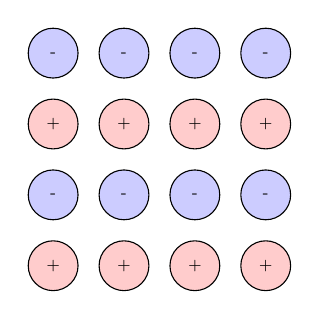
\begin{tikzpicture}[scale=0.9,
                    cation/.style={circle,draw=black,fill=white!80!red,minimum size=18},
                    anion/.style={circle,draw=black,fill=white!80!blue,minimum size=18}
                ]
                    \foreach \i in {1,...,2}
                        {
                        \foreach \j in {1,...,2}
                            {
                            \node[cation] (\i\j+) at (2*\i,2*\j) {\tiny{+}};
                            \node[anion] (\i\j+) at (2*\i,2*\j+1) {\tiny{-}};
                            \node[cation] (\i\j-) at (2*\i+1,2*\j) {\tiny{+}};
                            \node[anion] (\i\j-) at (2*\i+1,2*\j+1) {\tiny{-}};
                        }
                    }
                \end{tikzpicture}
                \caption{Type III (e.g., NaCl (111)).}
            \end{subfigure}
            \caption{Tasker classification of ionic crystals.\cite{taskerStabilityIonicCrystal1979}}
        \end{figure}

    \end{frame}


    \begin{frame}{Tasker III $\rightarrow$ Tasker 2b Reconstruction}
        \begin{figure}
            \centering
            \begin{subfigure}{0.3\textwidth}
                \centering
                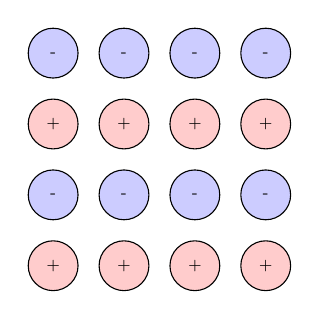
\begin{tikzpicture}[scale=0.9,
                    cation/.style={circle,draw=black,fill=white!80!red,minimum size=18},
                    anion/.style={circle,draw=black,fill=white!80!blue,minimum size=18}
                ]
                    \foreach \i in {1,...,2}
                        {
                        \foreach \j in {1,...,2}
                            {
                            \node[cation] (\i\j+) at (2*\i,2*\j) {\tiny{+}};
                            \node[anion] (\i\j+) at (2*\i,2*\j+1) {\tiny{-}};
                            \node[cation] (\i\j-) at (2*\i+1,2*\j) {\tiny{+}};
                            \node[anion] (\i\j-) at (2*\i+1,2*\j+1) {\tiny{-}};
                        }
                    }
                \end{tikzpicture}
                \caption{Type III.}
            \end{subfigure}
            \begin{subfigure}{0.3\textwidth}
                \centering
                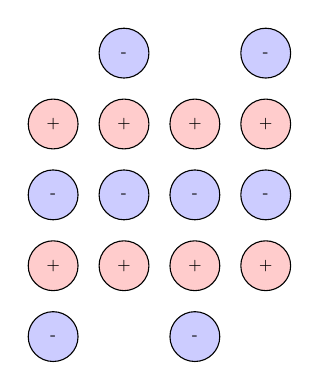
\begin{tikzpicture}[scale=0.9,
                    cation/.style={circle,draw=black,fill=white!80!red,minimum size=18},
                    anion/.style={circle,draw=black,fill=white!80!blue,minimum size=18}
                ]
                    \node[anion] () at (1, 0) {\tiny{-}};
                    \node[anion] () at (3, 0) {\tiny{-}};
                    \node[anion] () at (2, 4) {\tiny{-}};
                    \node[anion] () at (4, 4) {\tiny{-}};
                    \foreach \i in {1,...,4}
                        {
                        \node[cation] (\i+) at (\i,1) {\tiny{+}};
                        \node[anion] (\i+) at (\i,2) {\tiny{-}};
                        \node[cation] (\i-) at (\i,3) {\tiny{+}};
                    }
                \end{tikzpicture}
                \caption{Reconstructed Type IIb.}
            \end{subfigure}
            \caption{Move half of atoms from top layer to bottom layer to create non-polar surfaces.}
        \end{figure}

    \end{frame}

    \begin{frame}{Surface Reconstructions}
        \begin{figure}
            \centering
            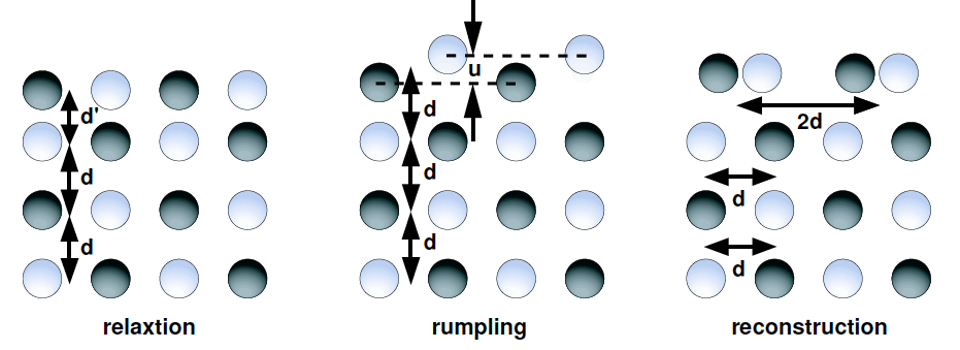
\includegraphics[width=0.9\linewidth]{lectures/figures/11_reconstructions.png}
        \end{figure}
    \end{frame}

    \begin{frame}{Si(111)-(7x7) – 25 years of science!}
        \begin{figure}
            \centering
            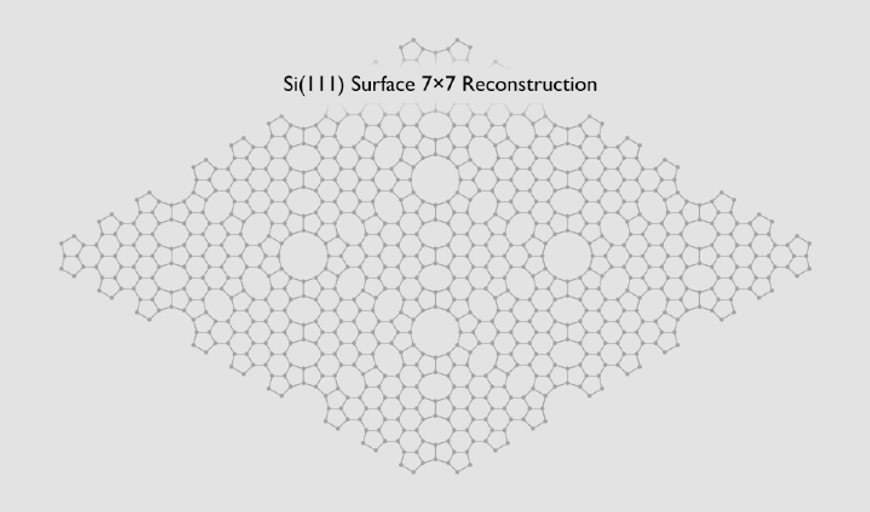
\includegraphics[width=0.7\linewidth]{lectures/figures/11_Si111.png}
            \caption{\url{https://vimeo.com/1086112}}
        \end{figure}
    \end{frame}

    \begin{frame}{Convergence of Surface Energies}
        \begin{columns}
            \column{0.3\textwidth}
            \begin{figure}
                \centering
                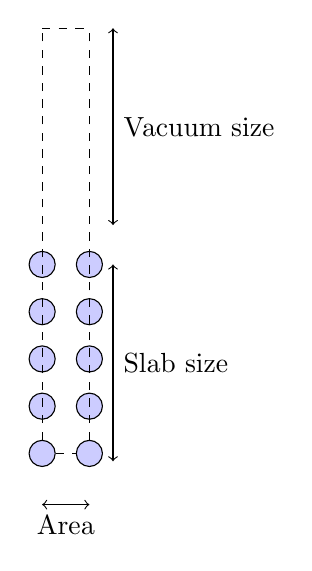
\begin{tikzpicture}[scale=0.5,
                    atom/.style={circle,draw=black,fill=white!80!blue,minimum size=5},
                    dopant/.style={circle,draw=black,fill=white!80!red,minimum size=5}
                ]
                    \foreach \i in {1,...,2}
                        {
                        \foreach \j in {1,...,5}
                            {
                            \pgfmathtruncatemacro{\label}{\i\j};
                            \node[atom] (\label) at (1.2*\i,1.2*\j) { };
                        }
                    }

                    \draw[dashed] (11) -- (1.2,12);
                    \draw[dashed] (11) -- (21);
                    \draw[dashed] (21) -- (2.4,12);
                    \draw[dashed] (1.2,12) -- (2.4,12);
                    \draw[<->] (3,1) -- node[right= 0.1mm] {Slab size} (3, 6);
                    \draw[<->] (3,7) -- node[right= 0.1mm] {Vacuum size} (3, 12);
                    \draw[<->] (1.2,-0.1) -- node[below= 0.1mm] {Area} (2.4, -0.1);

                \end{tikzpicture}
            \end{figure}
            \column{0.7\textwidth}
            \begin{equation*}
                \gamma = \frac{1}{2A} [ E(\mathrm{slab})-NE(\mathrm{bulk})]
            \end{equation*}

            Most people remember convergence wrt vacuum and slab size, but convergence wrt surface area can be important, particularly if there are reconstructions that can break symmetry!

            \begin{figure}
                \centering
                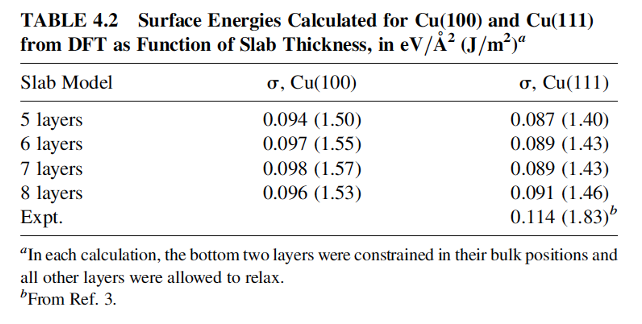
\includegraphics[width=0.6\linewidth]{lectures/figures/11_Cu_surface_energies.png}
                \caption{\cite{shollDensityFunctionalTheory2023}}
            \end{figure}

        \end{columns}
    \end{frame}


    \begin{frame}{Practical Aspects of Surface Calculations - Cells and $k$ points}
        \begin{columns}
            \column{0.5\textwidth}
            \begin{figure}
                \centering
                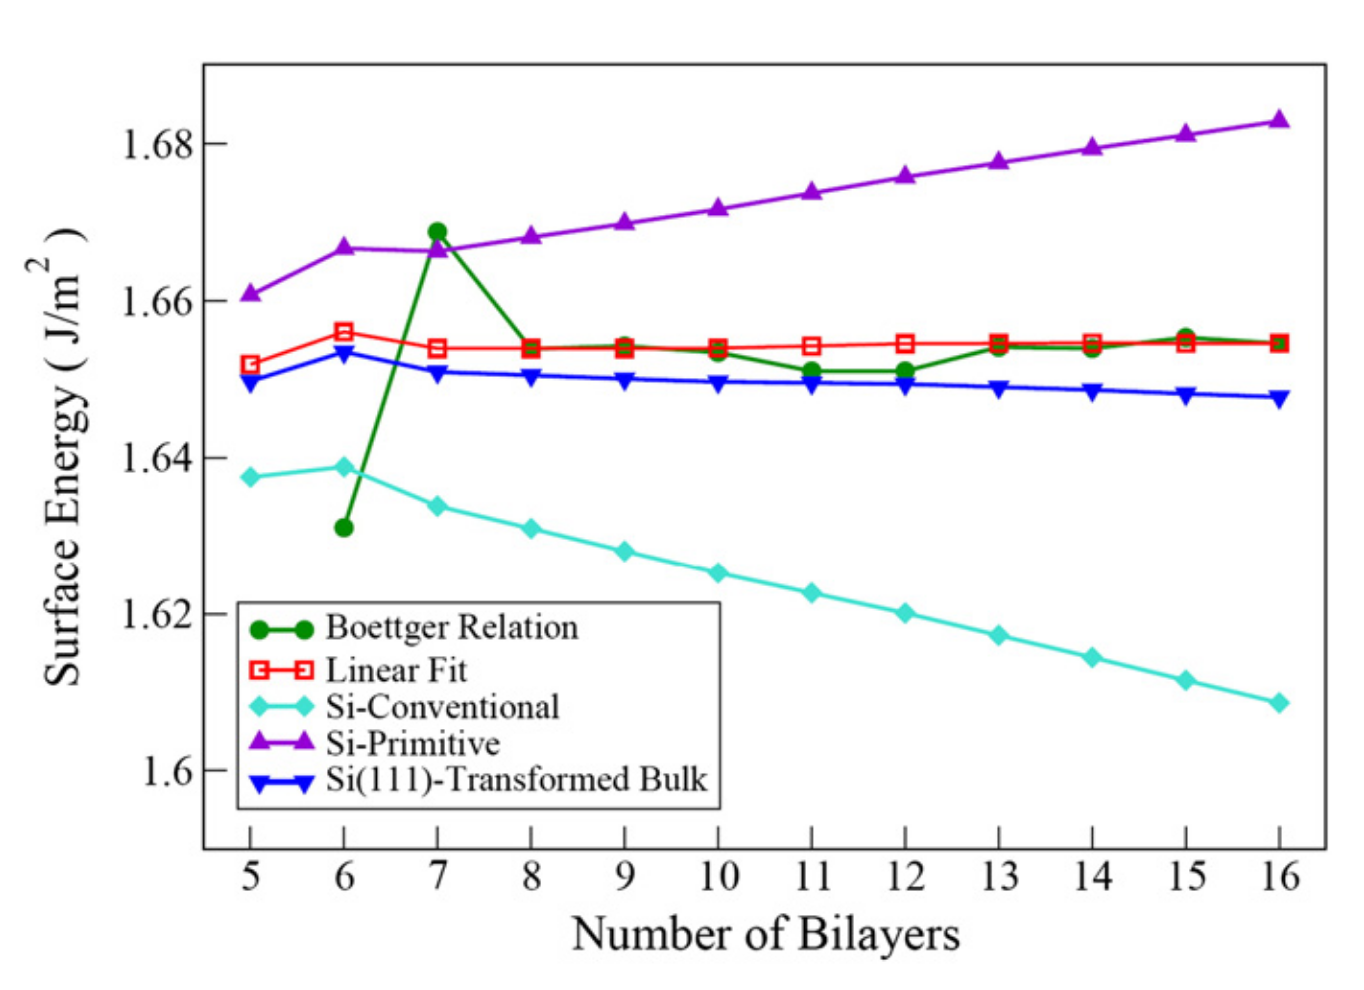
\includegraphics[width=\linewidth]{lectures/figures/11_surface_kpoints.png}
                \caption{Surface energies calculated using five different bulk energy values.\cite{sunEfficientCreationConvergence2013}}
            \end{figure}
            \column{0.5\textwidth}
            \begin{itemize}
                \item Surface Brillouin Zone is 2D $\implies$ only single $k$ point used in direction normal to slab.
                \item Consistent $k$-point meshes should be used for bulk and surface calculations to ensure cancellation of errors and convergence of surface energy.
                \item Scheme recommended by \cite{sunEfficientCreationConvergence2013} - compute bulk energy using transformed unit cell and consistent $k$-point mesh, $7 \times 7 \times 7$ for bulk Si and $7 \times 7 \times 1$ for slab.
            \end{itemize}
        \end{columns}

    \end{frame}

    \begin{frame}{Practical Aspects of Surface Calculations - Functionals}
        \begin{figure}
            \centering
            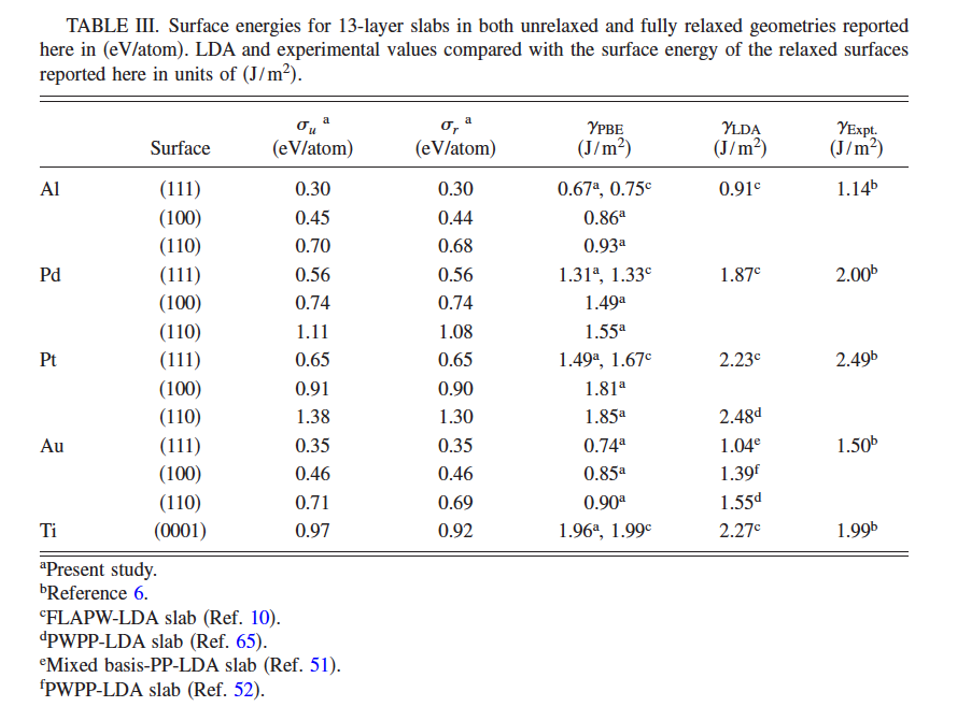
\includegraphics[width=0.5\linewidth]{lectures/figures/11_surface_functionals.png}
            \caption{LDA outperforms PBE for some surfaces.\cite{singh-millerSurfaceEnergiesWork2009}.}
        \end{figure}
    \end{frame}

    \begin{frame}{Absorbates on Surfaces}
        \begin{figure}
            \centering
            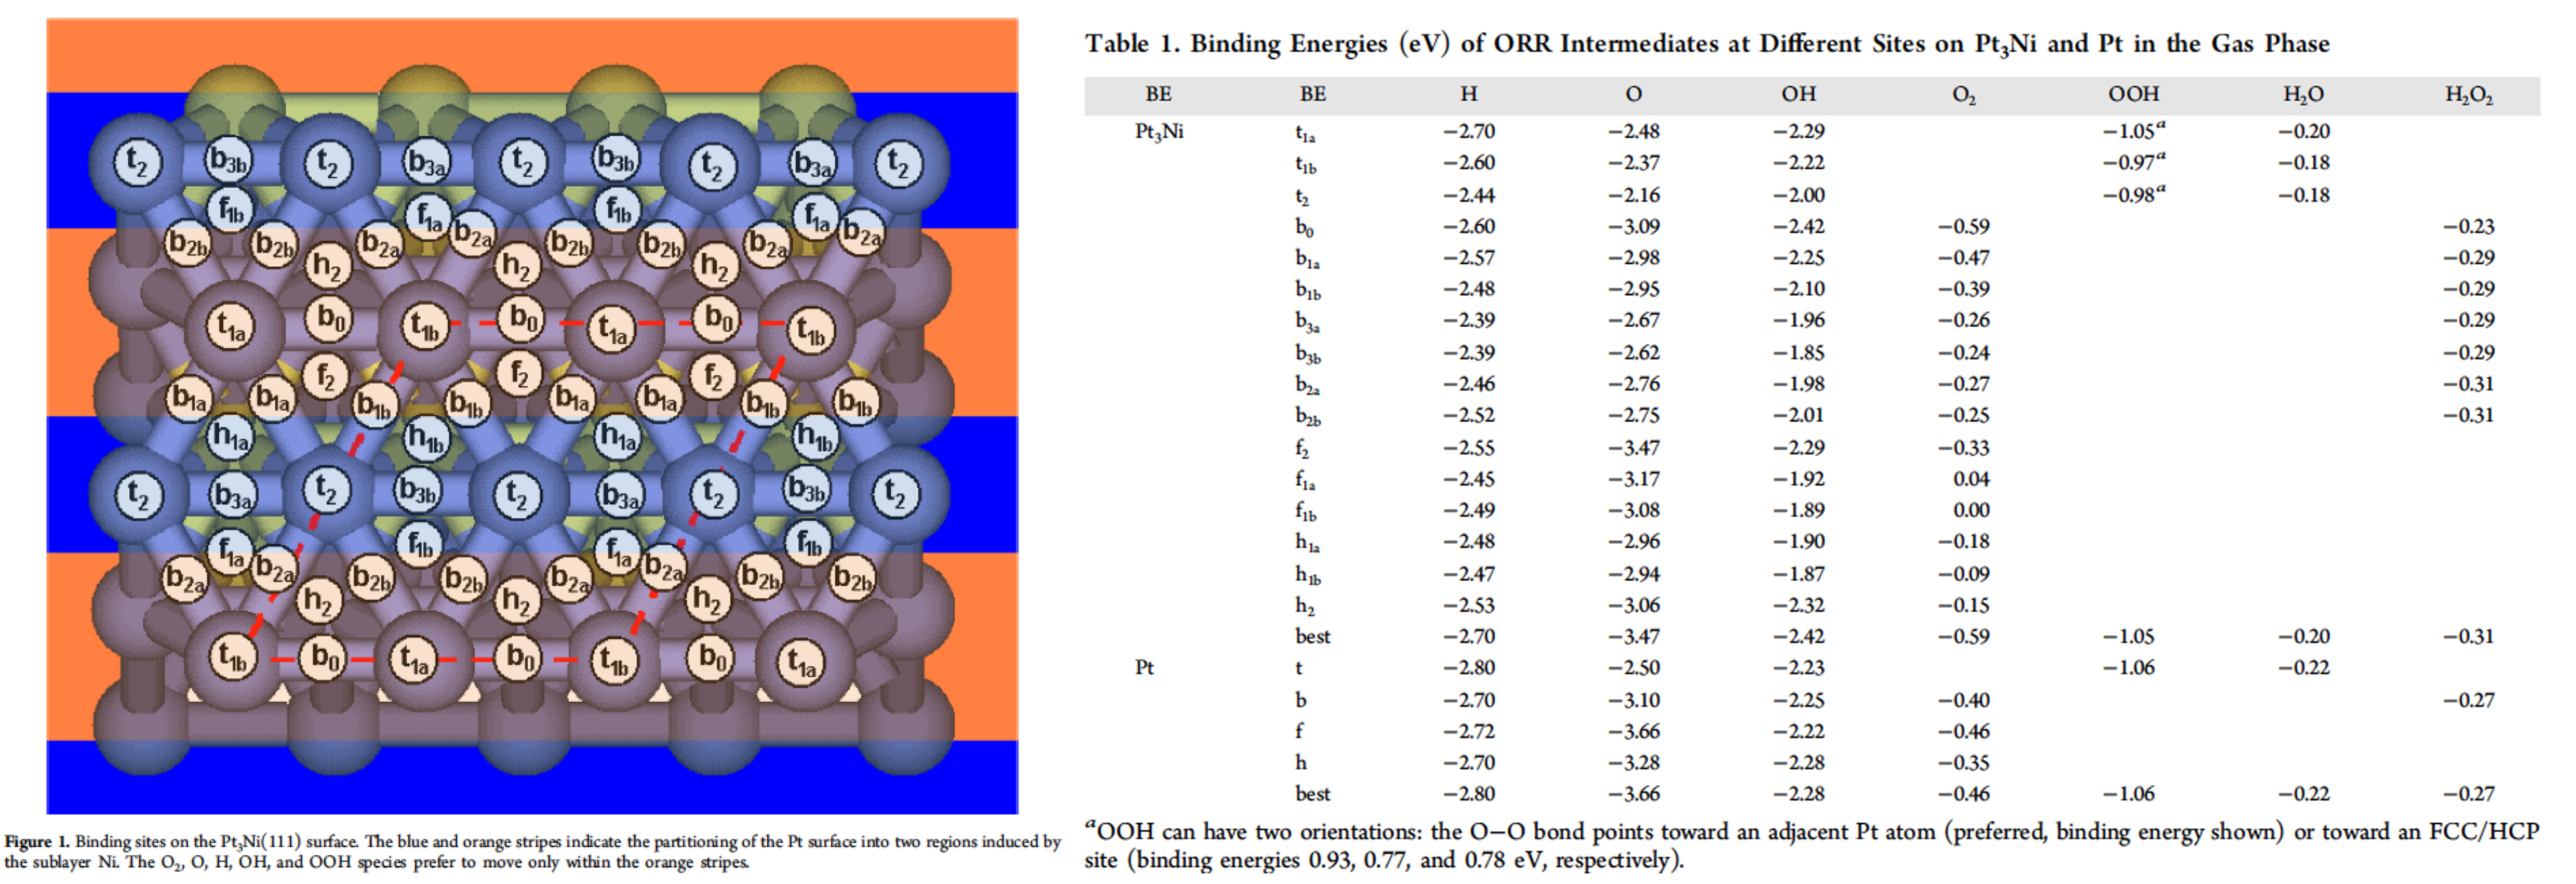
\includegraphics[width=\linewidth]{lectures/figures/11_binding.png}
            \caption{Mechanism for Oxygen Reduction Reaction on \ce{Pt3Ni} Fuel Cell Cathode.\cite{shaMechanismOxygenReduction2012}}
        \end{figure}
    \end{frame}


    \begin{frame}{Applications: Catalysis}
        \begin{figure}
            \centering
            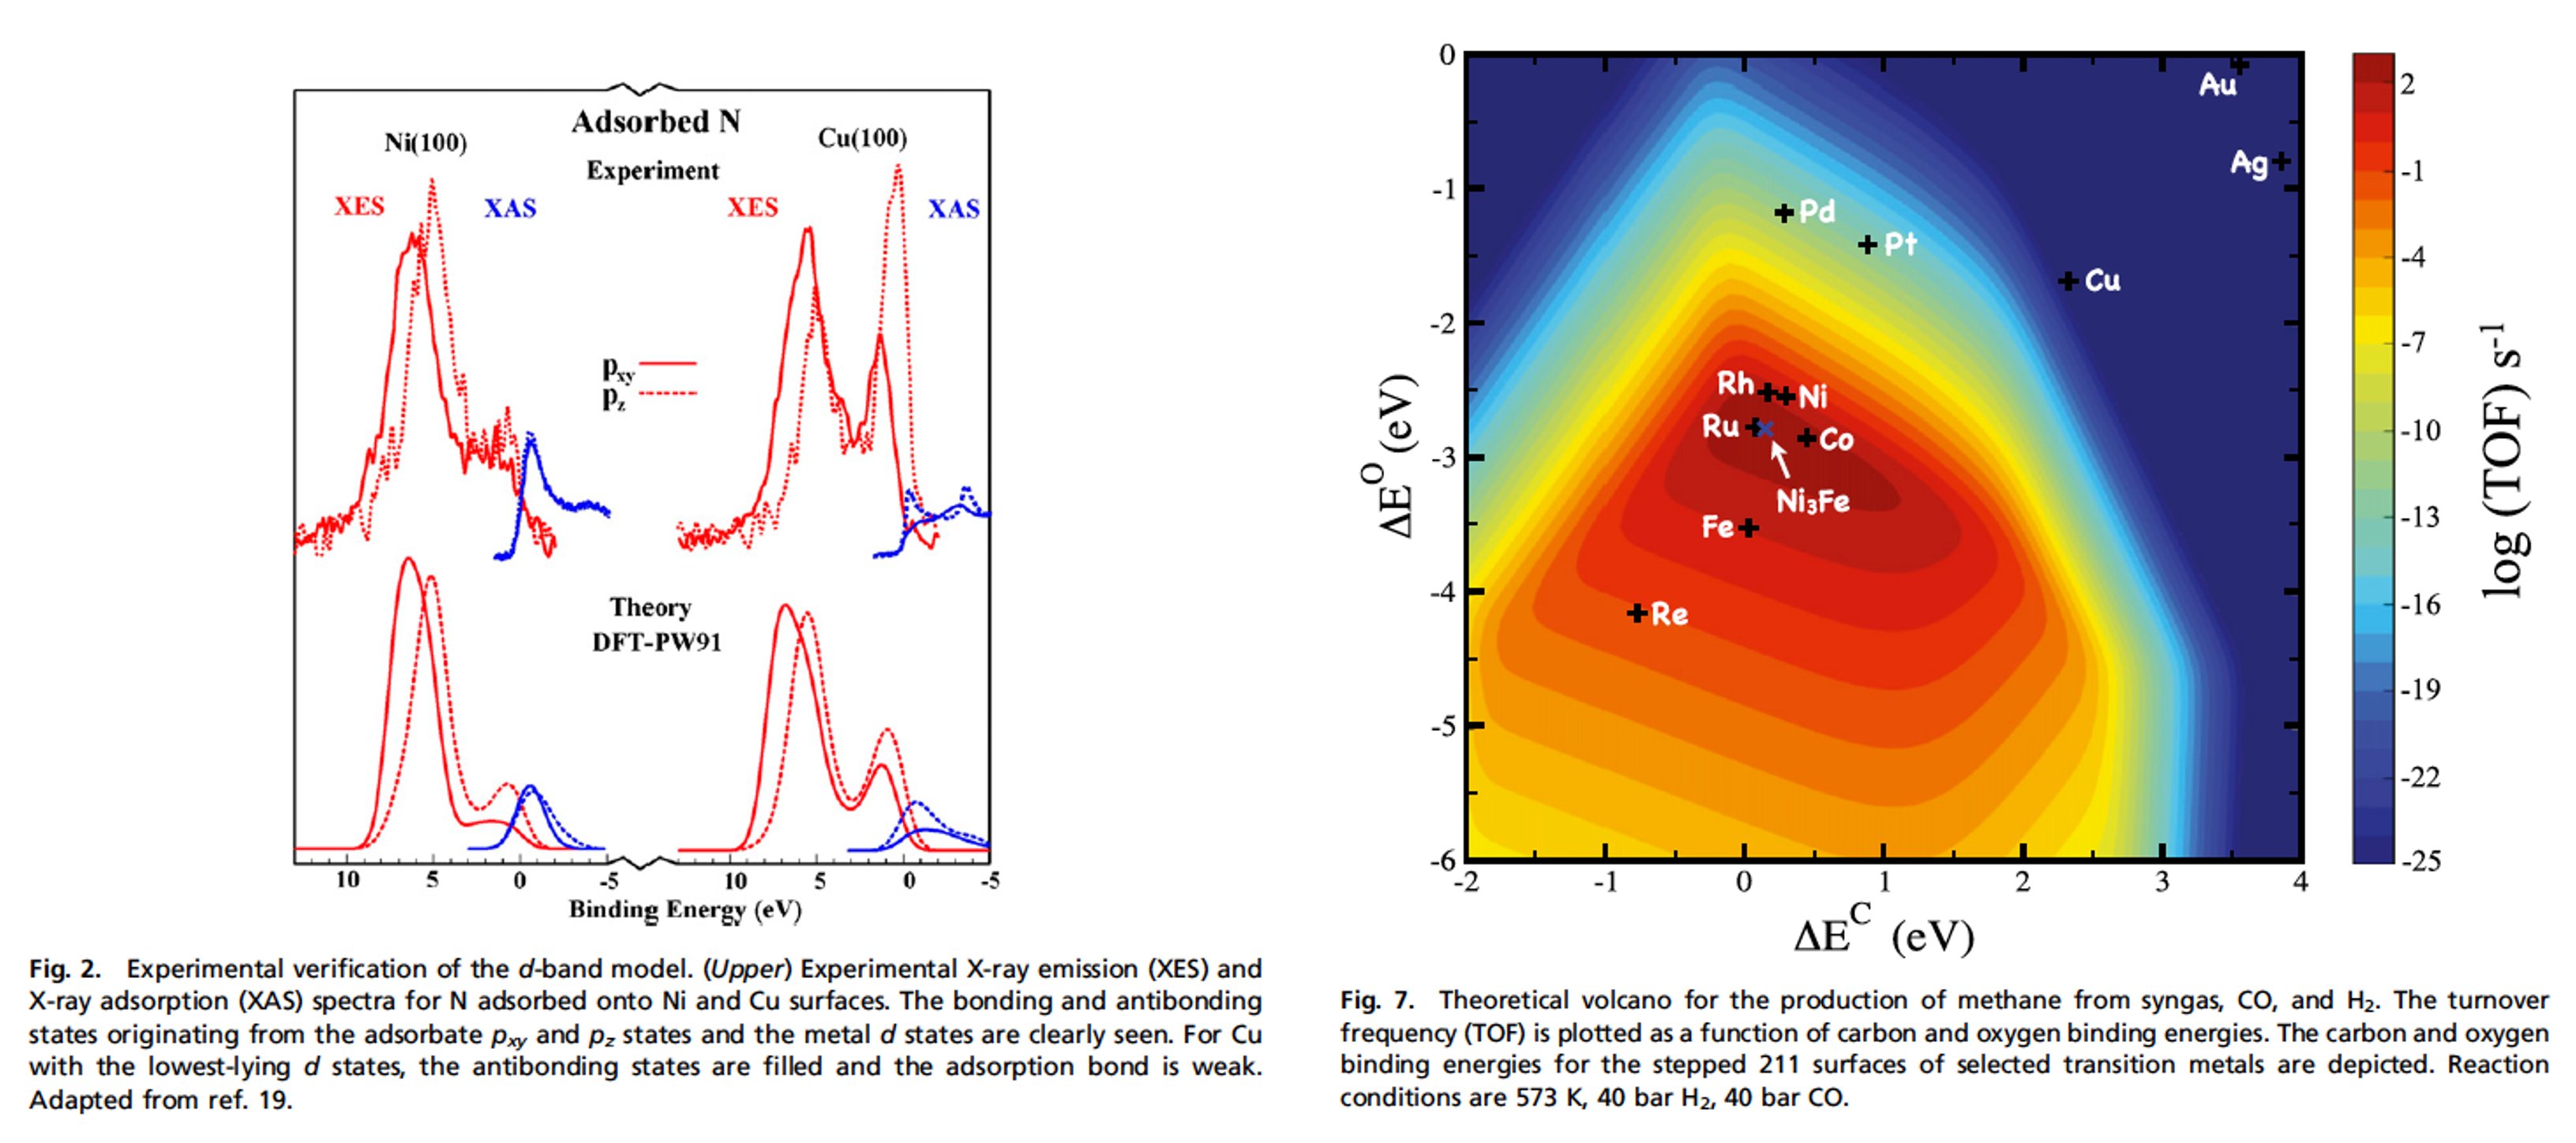
\includegraphics[width=0.8\linewidth]{lectures/figures/11_catalysis.png}
            \caption{The d-band model and volcano plot.\cite{norskovSurfaceChemistrySpecial2011}}
        \end{figure}
    \end{frame}

    \begin{frame}{Applications: Metastability and Synthesizability}

        \begin{figure}
            \centering
            \begin{subfigure}{0.45\textwidth}
                \centering
                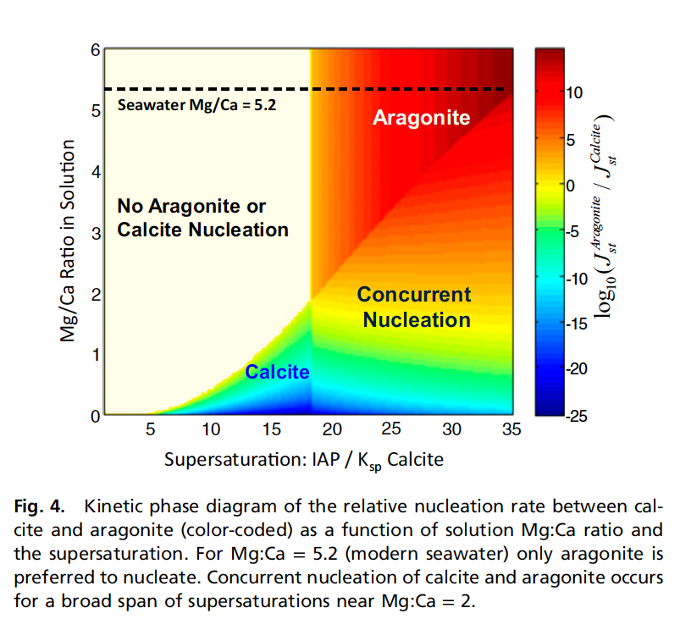
\includegraphics[width=\linewidth]{lectures/figures/11_metastable.png}
                \caption{\cite{sunCorrectionSunNucleation2015}}
            \end{subfigure}
            \begin{subfigure}{0.45\textwidth}
                \centering
                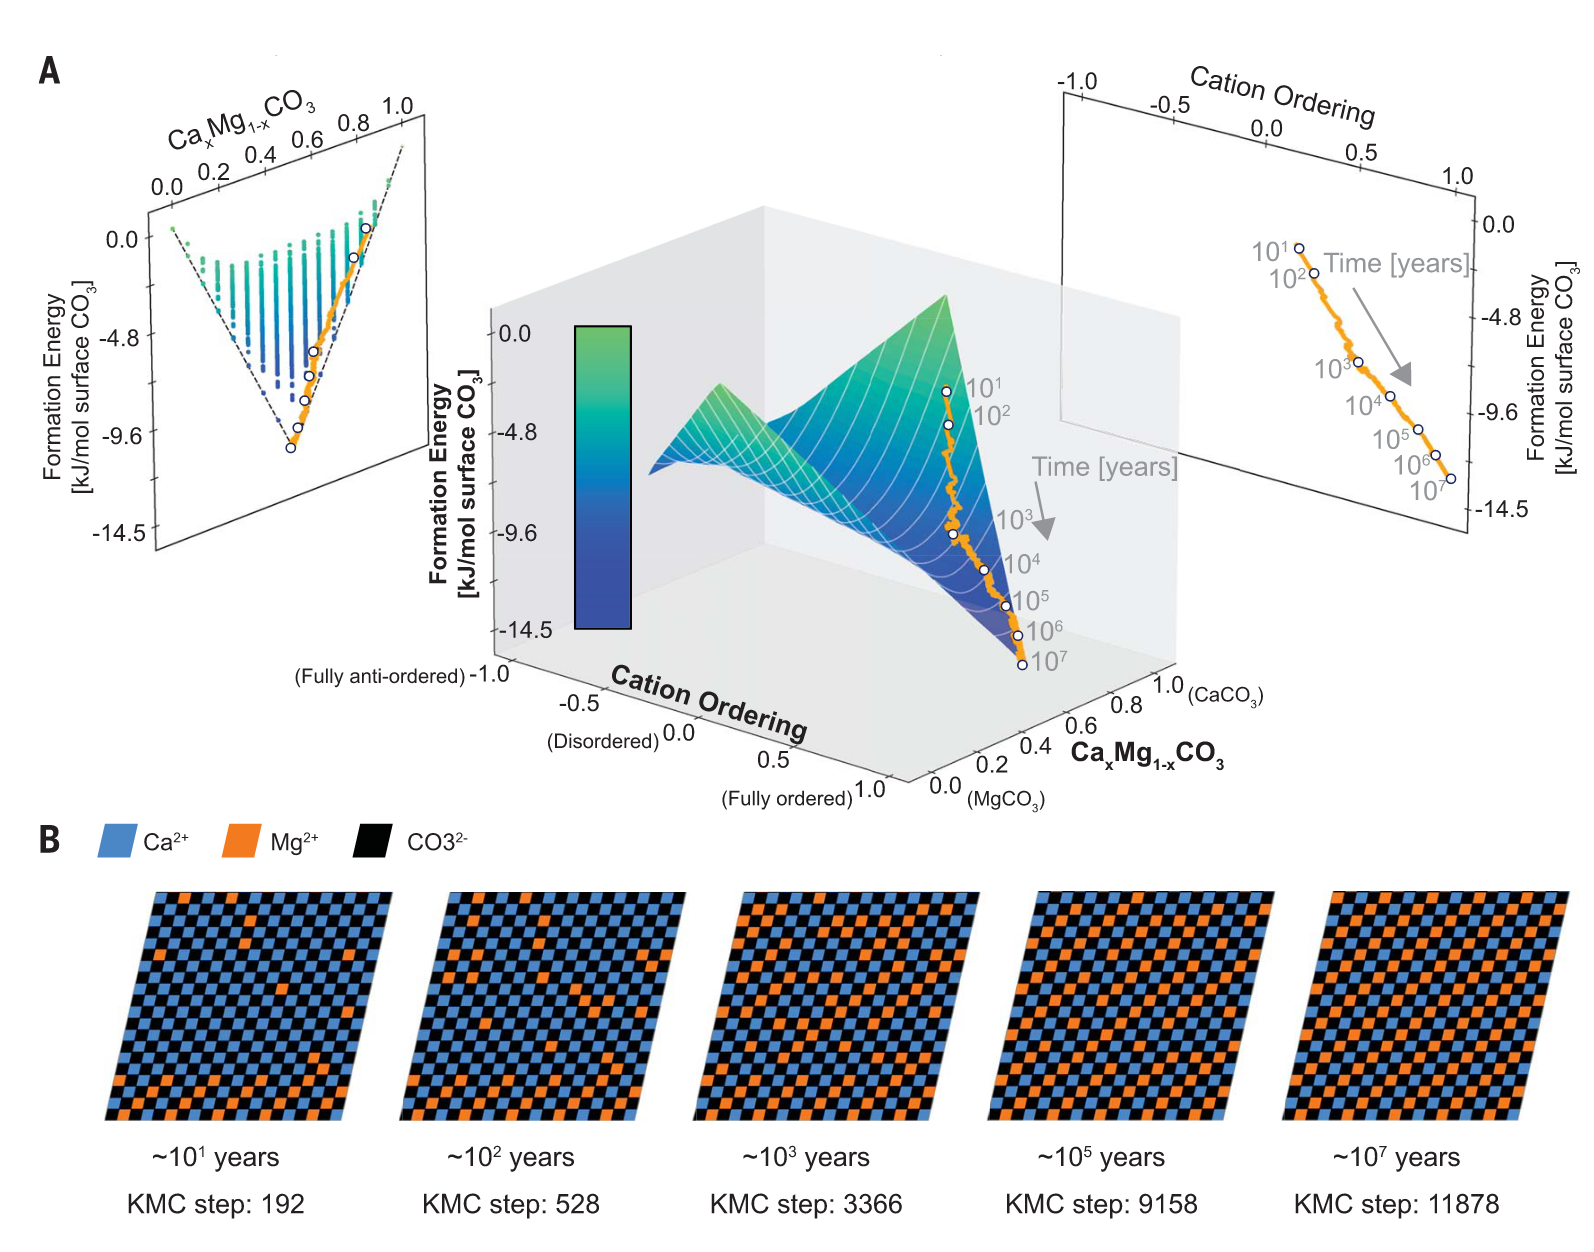
\includegraphics[width=0.9\linewidth]{lectures/figures/11_dolomite.png}
                \caption{Dolomite step-edge growth and ordering through dissolution-reprecipitation under constant supersaturation as simulated with kinetic Monte Carlo.\cite{kimDissolutionEnablesDolomite2023}}
            \end{subfigure}
        \end{figure}

    \end{frame}


    \begin{frame}{Interfaces}
        \begin{figure}
            \centering
            \begin{subfigure}{0.45\textwidth}
                \centering
                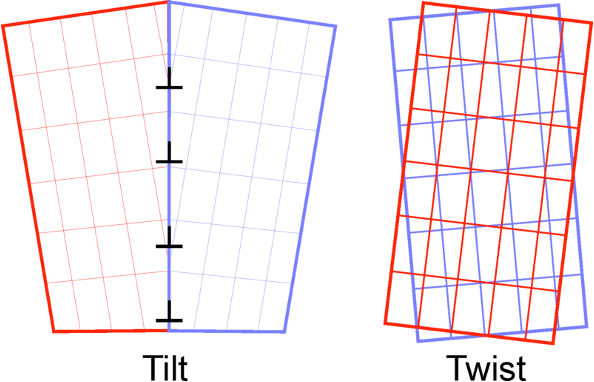
\includegraphics[width=\linewidth]{lectures/figures/11_GBs.png}
                \caption{Grain Boundaries}
            \end{subfigure}
            \begin{subfigure}{0.45\textwidth}
                \centering
                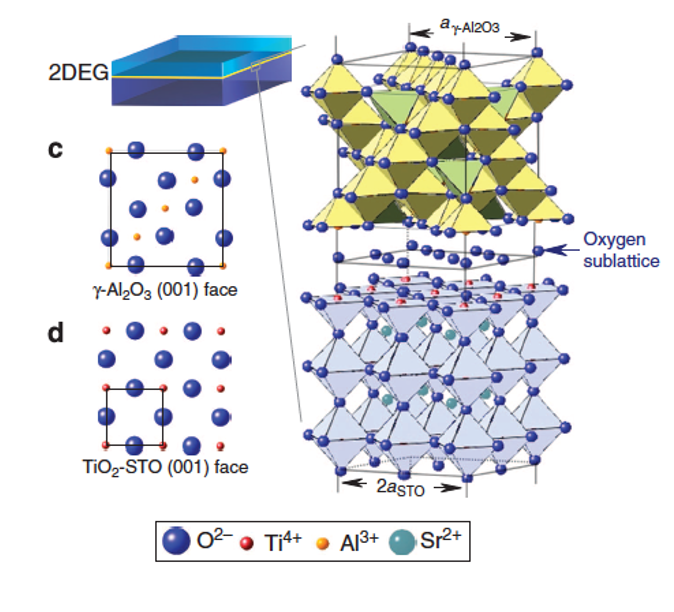
\includegraphics[width=\linewidth]{lectures/figures/11_hetero_interfaces.png}
                \caption{Hetereogenous solid-solid interfaces.}
            \end{subfigure}
        \end{figure}
    \end{frame}

    \begin{frame}{Liquid metal embrittlement in Ni}
        \begin{figure}
            \centering
            \begin{subfigure}{0.45\textwidth}
                \centering
                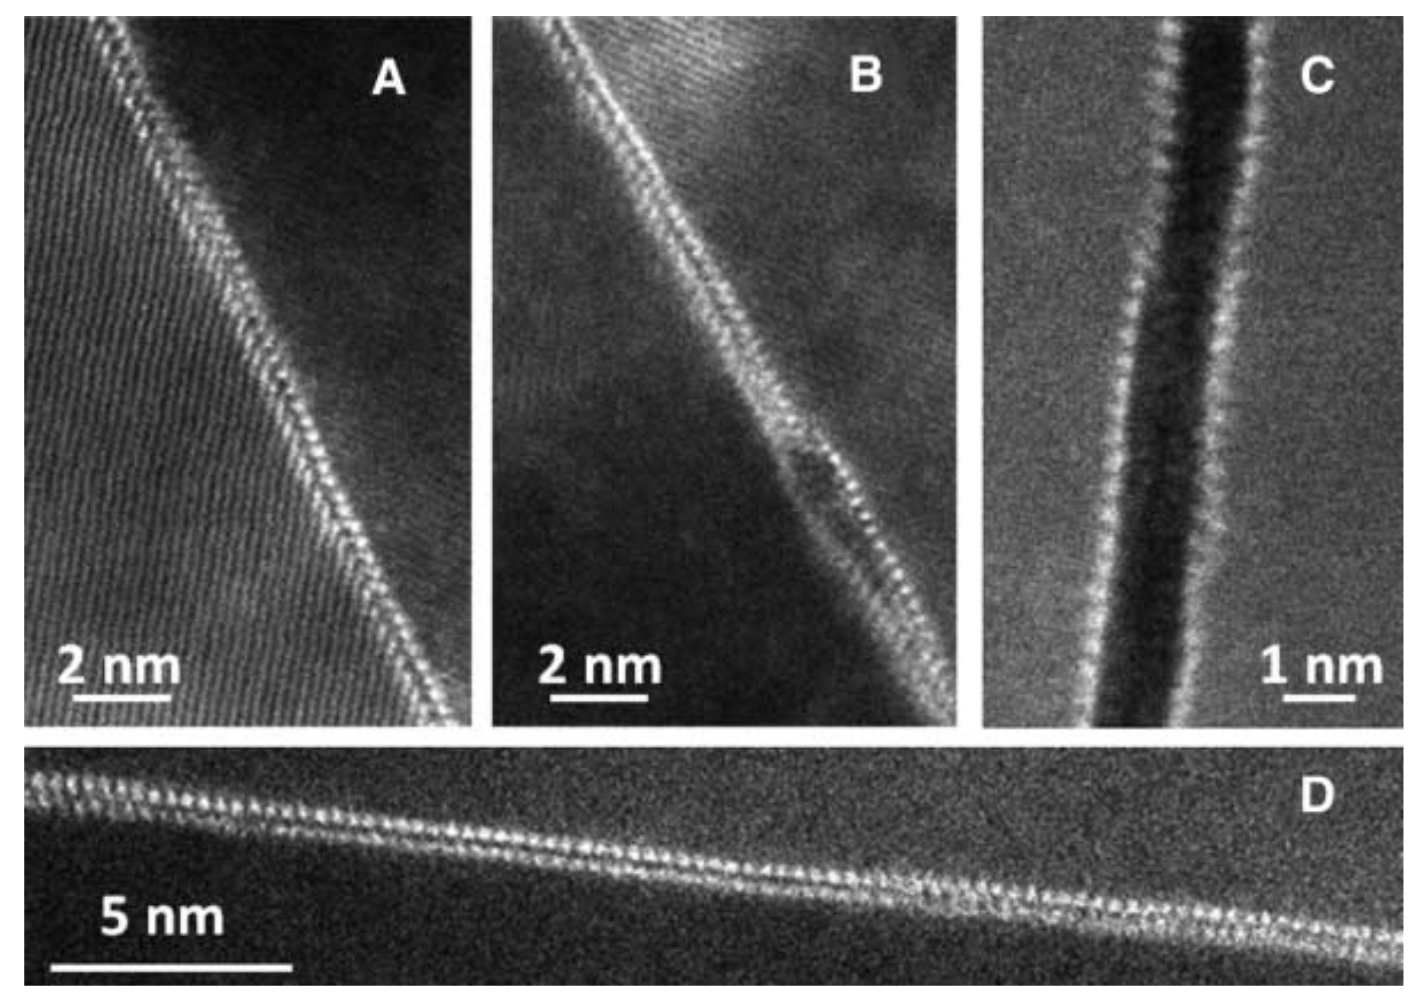
\includegraphics[width=\linewidth]{lectures/figures/11_Bi_in_Ni.png}
                \caption{STEM HAADF micrographs showing two layers of Bi absorbed along the general GBs of a Ni polycrystal quenched from 700$^o$C. The weakly bonded Bi atoms cause the boundaries to easily fracture between the layers.\cite{luoRoleBilayerInterfacial2011}}
            \end{subfigure}
            \begin{subfigure}{0.45\textwidth}
                \centering
                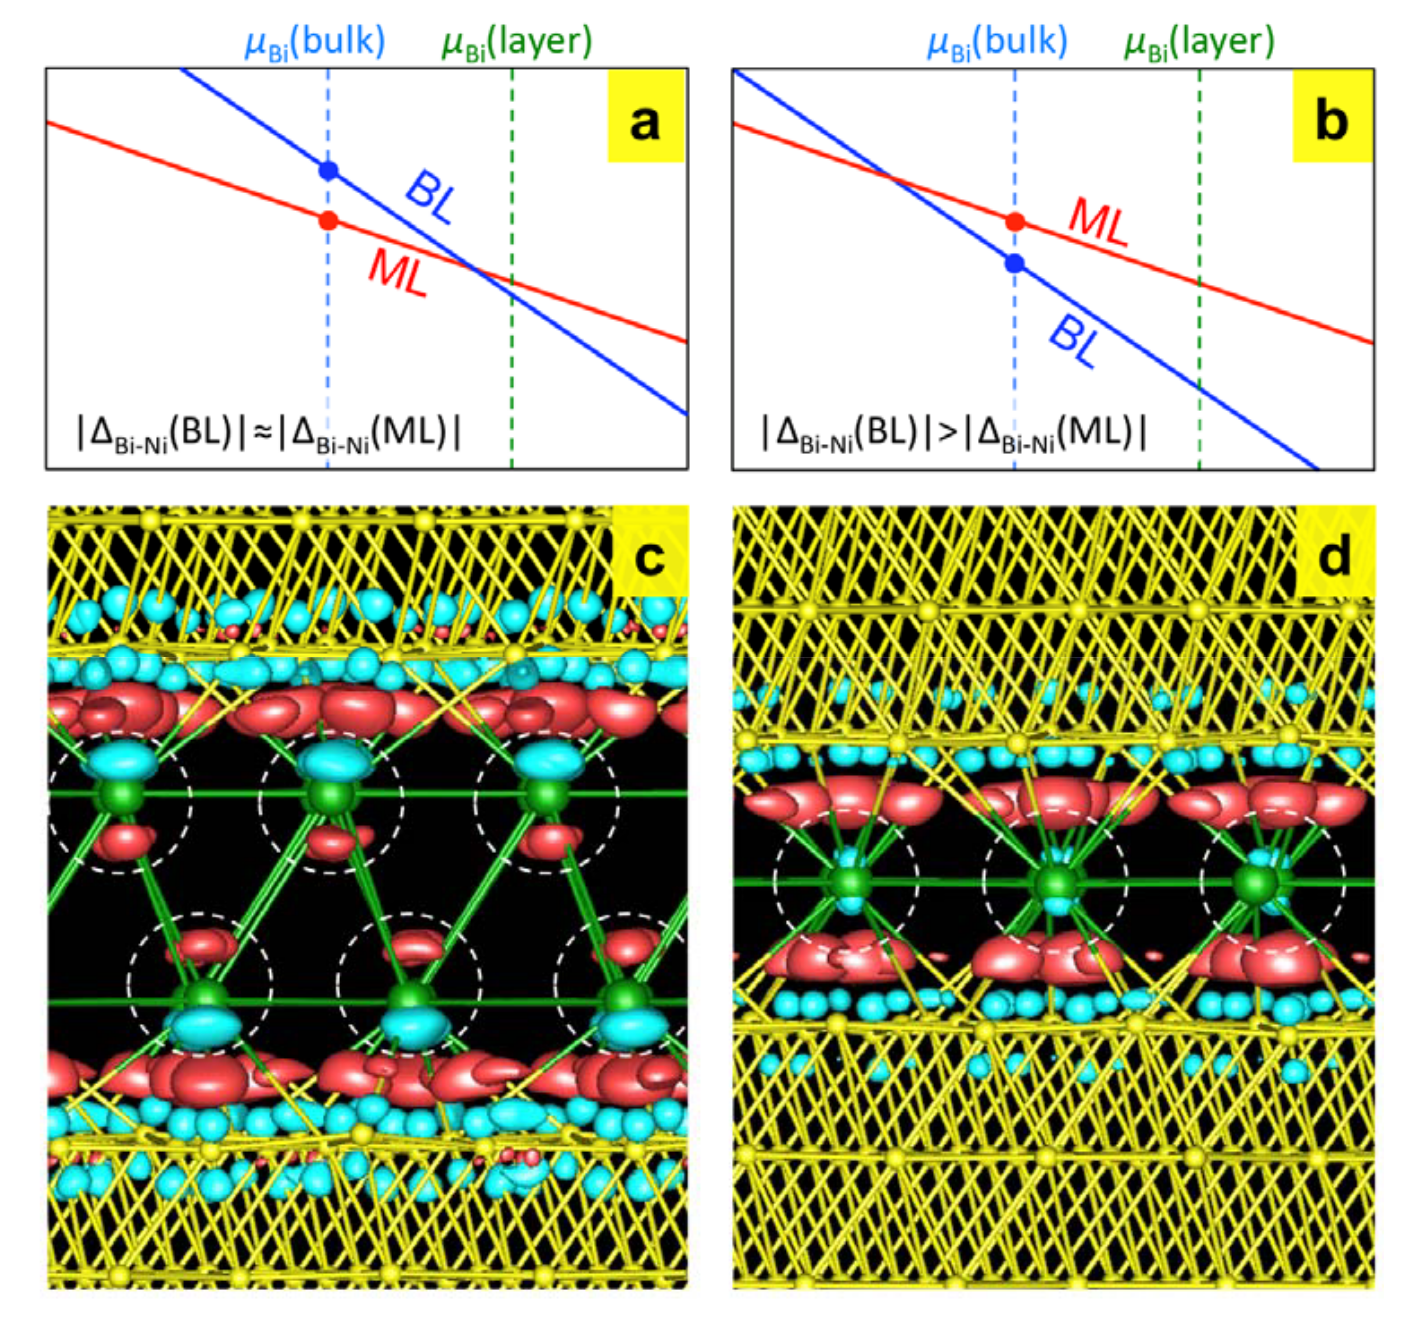
\includegraphics[width=0.8\linewidth]{lectures/figures/11_Bi_in_Ni_DFT.png}
                \caption{Relative stability of the Bi ML and BL in Ni GB as a function of the Bi chemical potential.\cite{kangOriginBismuthInducedDecohesion2013}}
            \end{subfigure}
        \end{figure}
    \end{frame}

    \begin{frame}{Solutes at Fe GBs}
        \begin{figure}
            \centering
            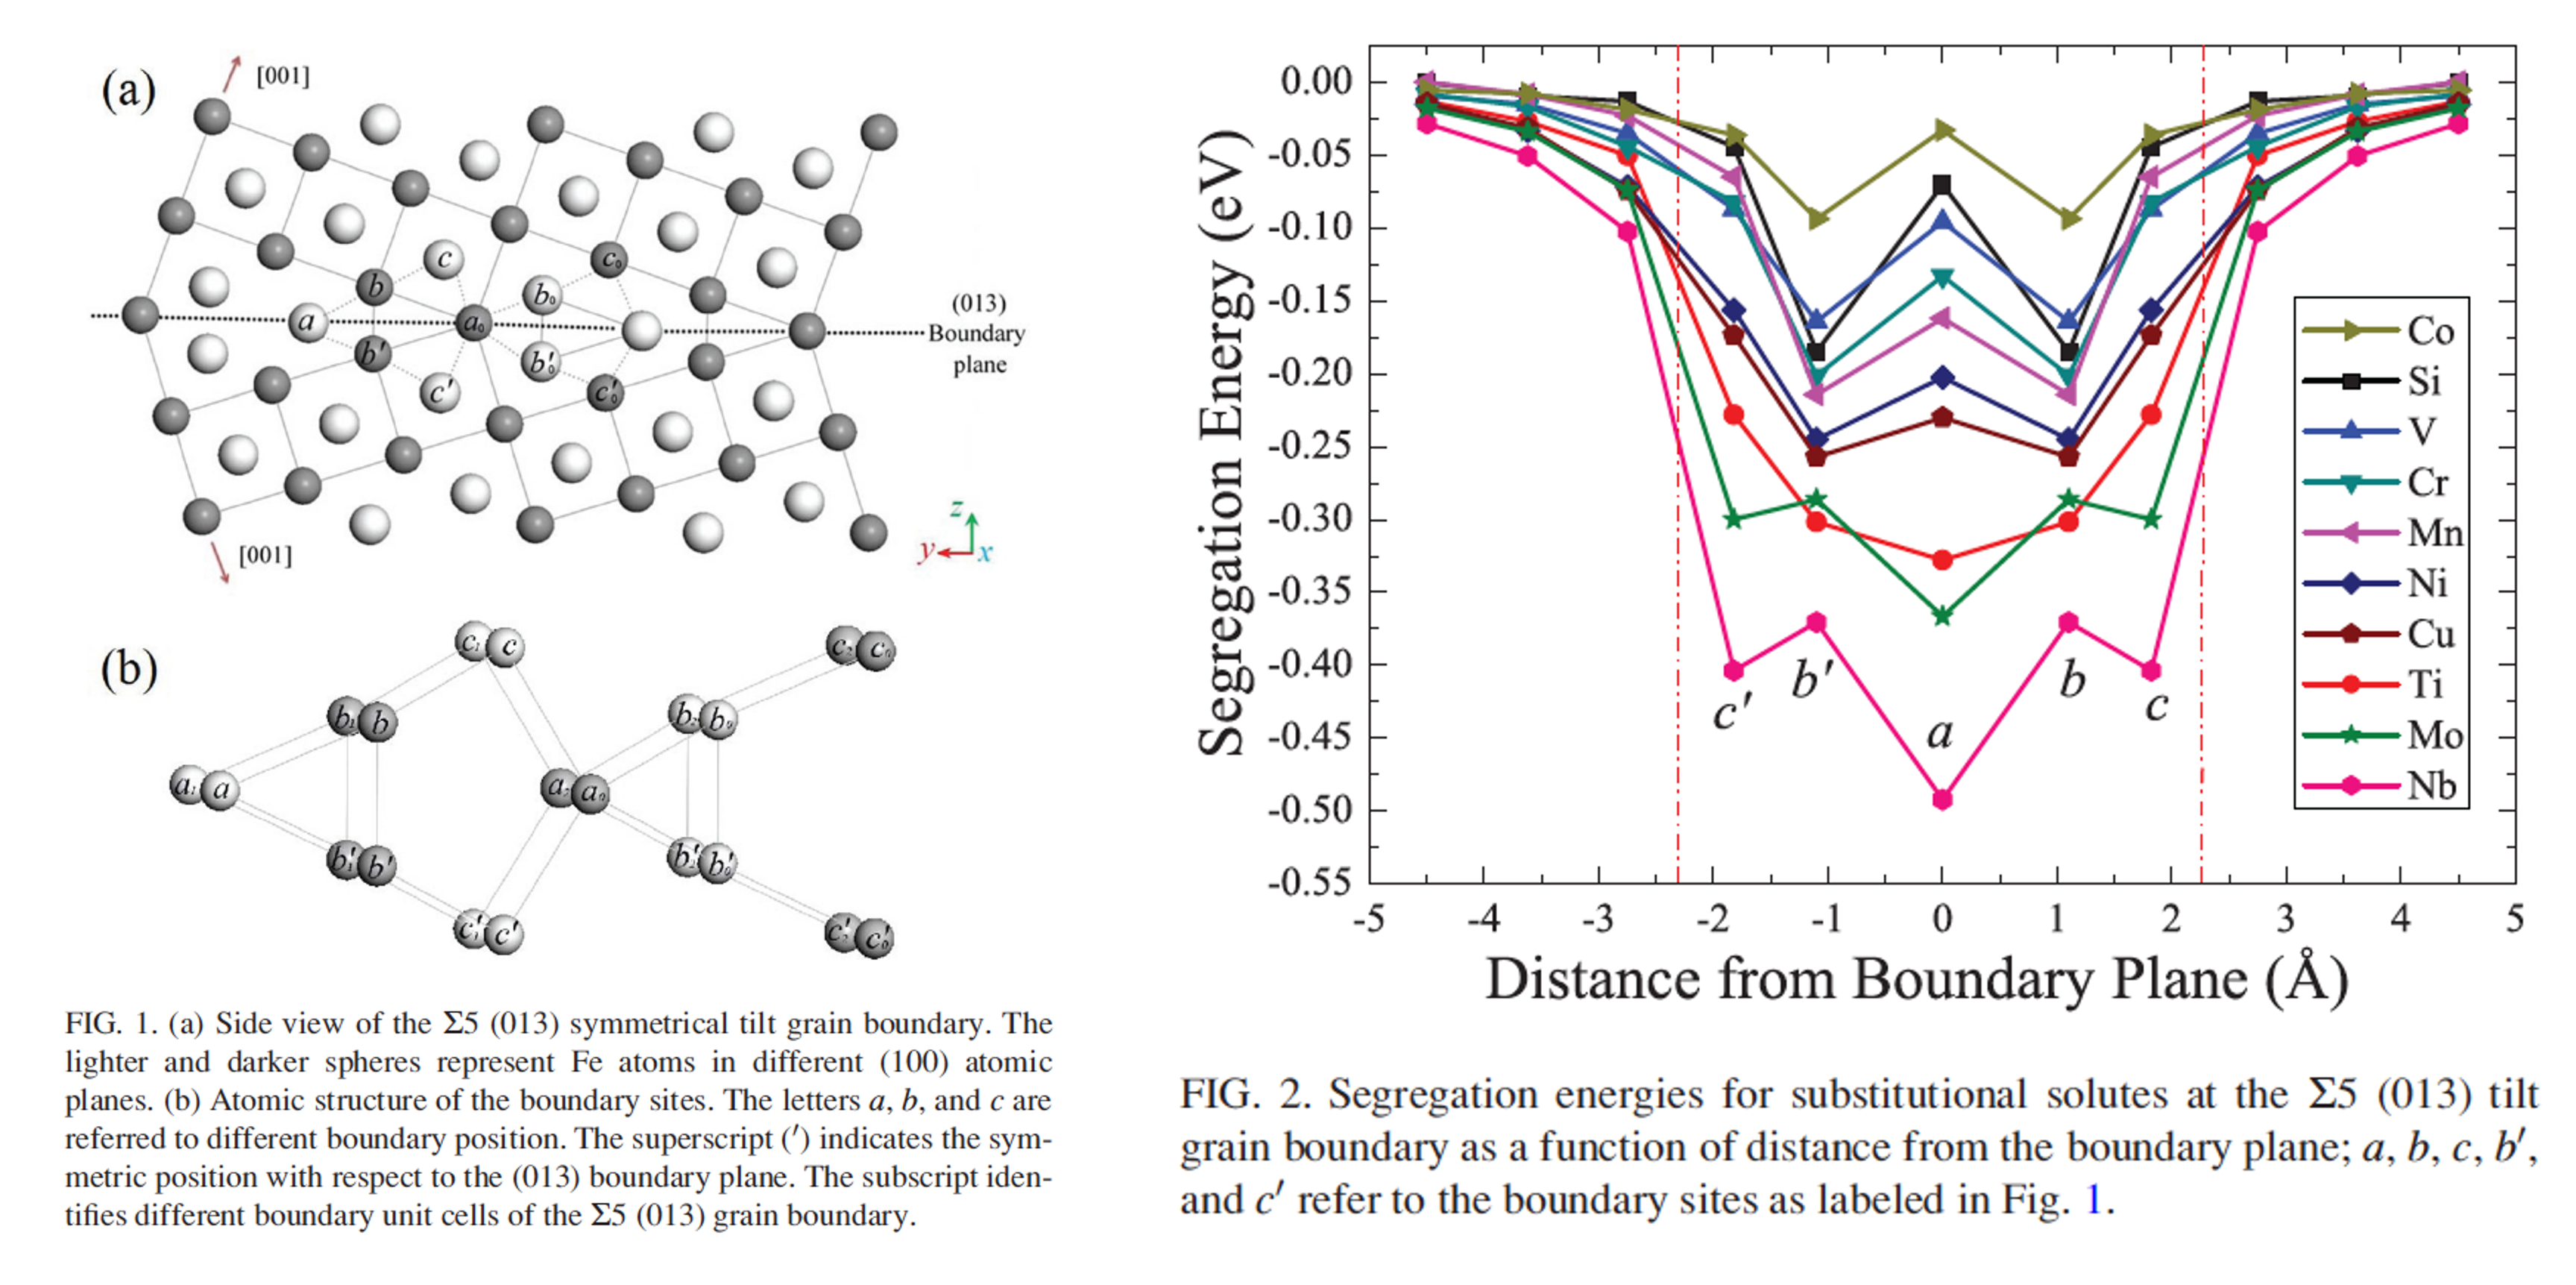
\includegraphics[width=0.8\linewidth]{lectures/figures/11_Solutes_at_Fe_GBs.png}
            \caption{From \cite{jinStudyInteractionSolutes2014}.}
        \end{figure}
    \end{frame}


    \begin{frame}{High-throughput Surfaces and GBs}
        \begin{figure}
            \centering
            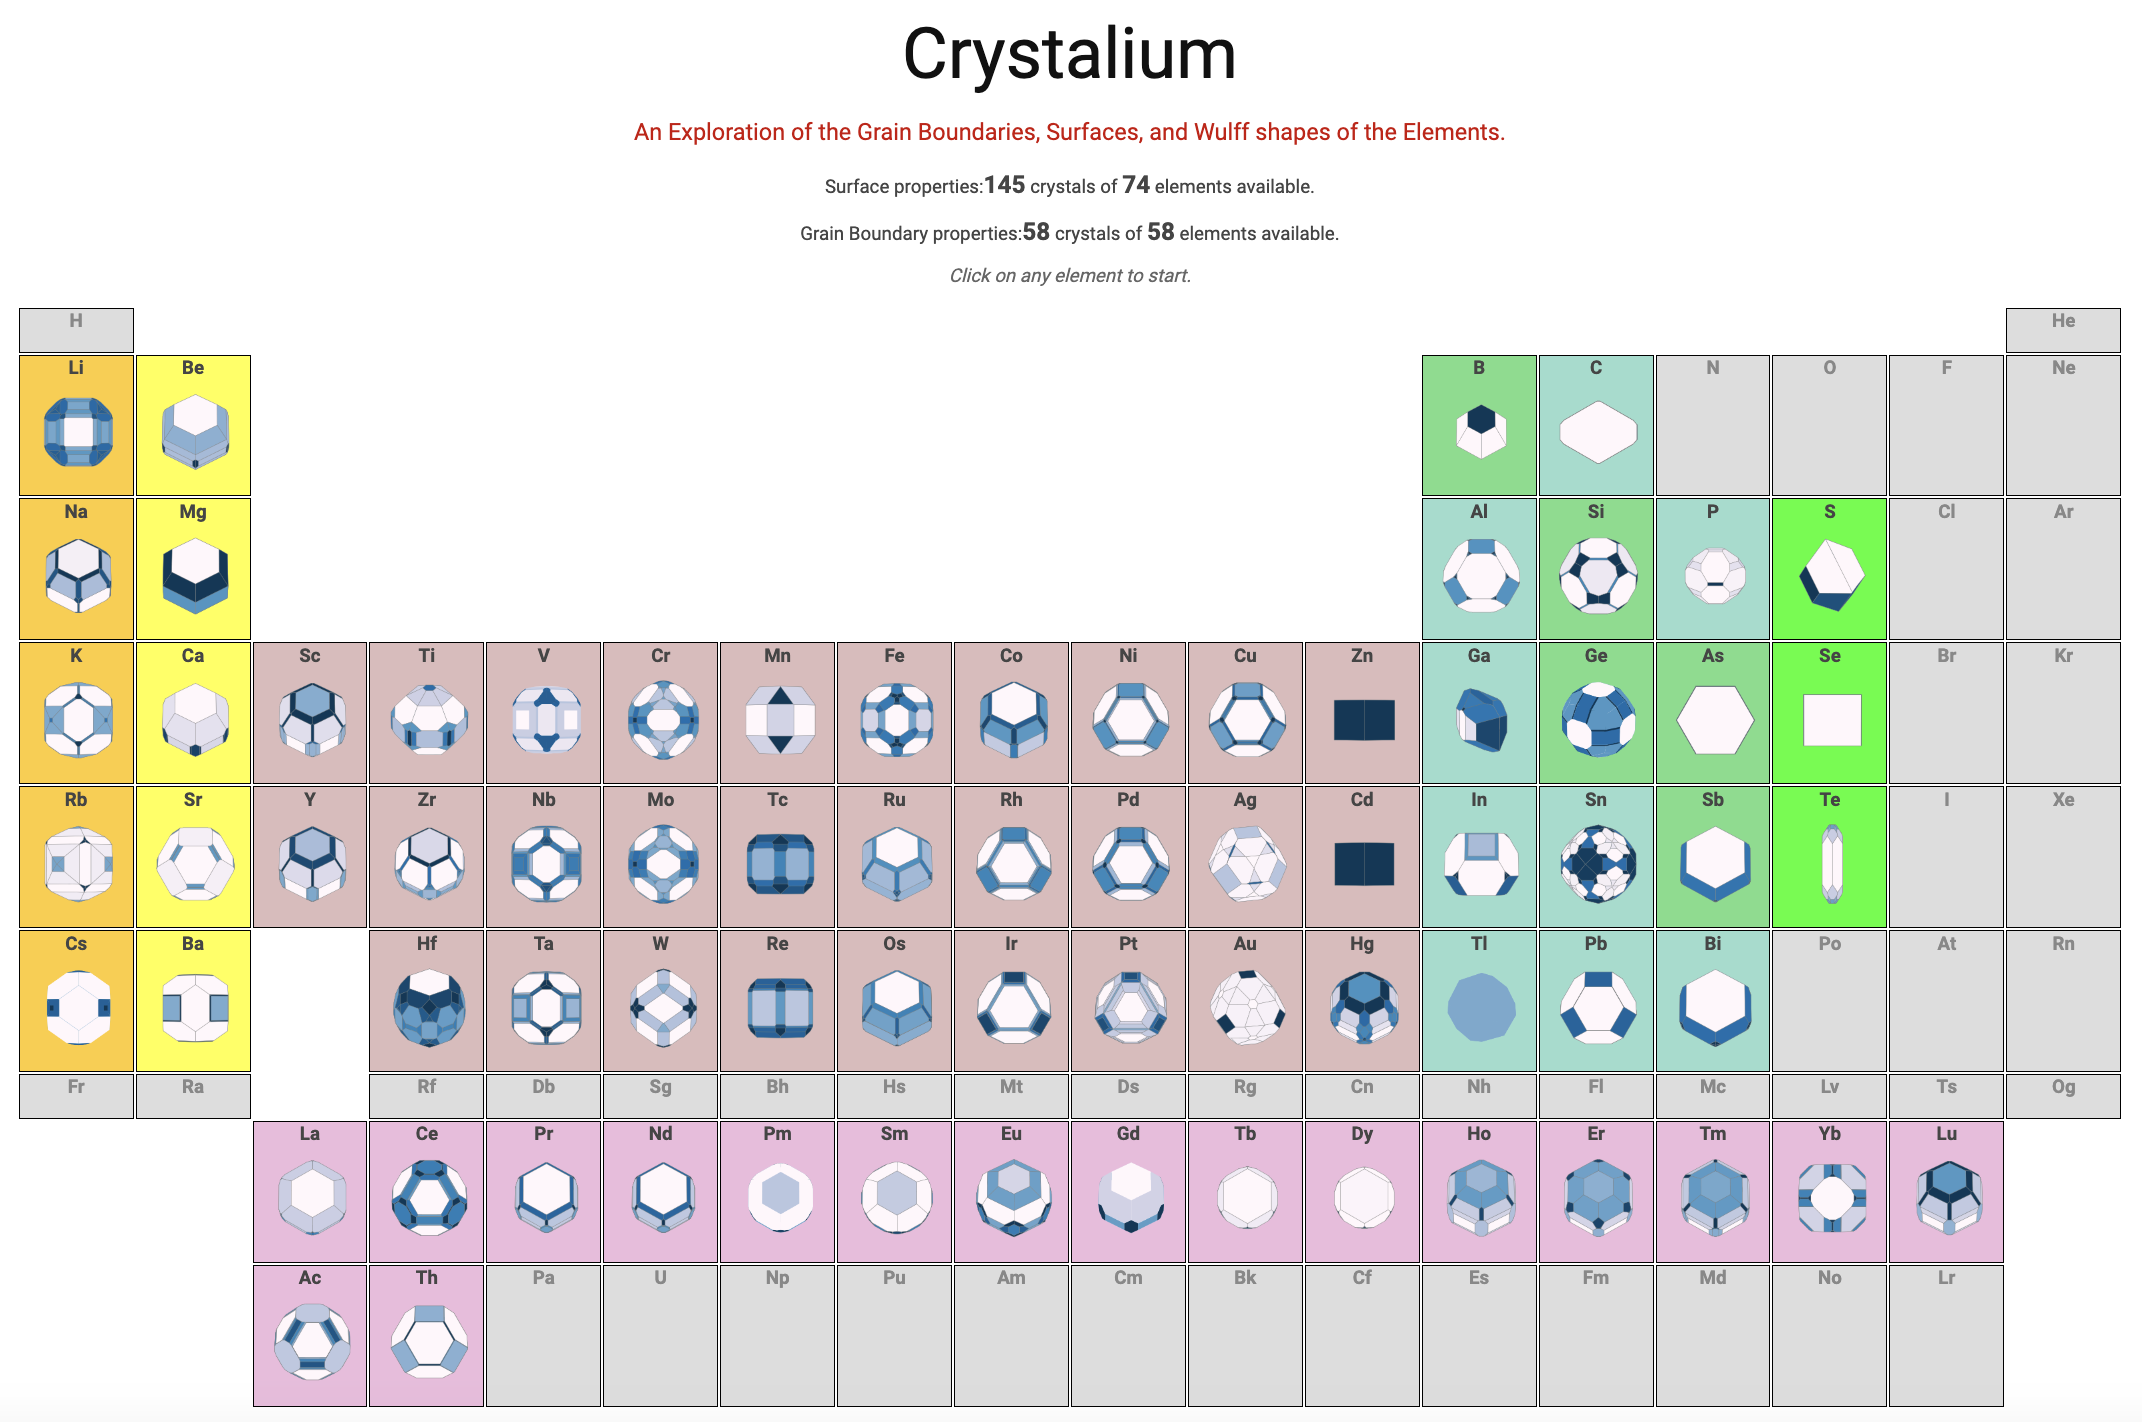
\includegraphics[width=0.5\linewidth]{lectures/figures/11_Crystalium.png}
            \caption{\url{http://crystalium.materialsvirtuallab.org}.\cite{tranSurfaceEnergiesElemental2016,tranAnisotropicWorkFunction2019,zhengGrainBoundaryProperties2020}}
        \end{figure}
    \end{frame}

    \begin{frame}[allowframebreaks]{Bibliography}
        \bibliographystyle{unsrt}
        \bibliography{refs}
    \end{frame}



    \begin{frame}
        \Huge{\centerline{The End}}
    \end{frame}

\end{document}

